The work developed in this chapter is quite independent 
from the main theme of this thesis, namely the problem of
\textit{Decision Making under Uncertainty}.
This work, performed in collaboration with Sergio Pizziol
and extending the work of his PhD thesis \cite{SERGIOTHESIS}, 
contributes to modelling human-machine interactions.
It is part of this thesis since it is a significant example of 
the need of qualitative models (such as those presented in previous chapters)
in some practical situations.

We formalize here a framework providing an estimate 
of the human assessment of the machine state, 
an automated detection of human operator attentional errors, 
and finally an estimate of the most plausible causes of these errors.
A qualitative possibilistic approach is used to deal 
with uncertainty about the human operator assessment. 

The human-machine context is first introduced to point out the need 
for a new modelling method for human attentional error.
Then a human error model is derived from the machine logic, using expert assumptions on human errors and their plausibility.
A human-machine interaction model results from the combination of the machine logic and the error model.
Using the Possibility Theory, an analysis model estimating the human assessment 
is built on the interaction model, summed up in a \textit{Possibilistic Hidden Markov Processes} ($\pi$-HMPs).
The possibilistic analysis is first performed on a toy example. 
Finally the soundness of the approach is shown through simulation tests 
with pilots performing a flight mission.

% Note that keywords are not normally used for peerreview papers.
%Human-Machine Interaction, Possibility Theory, Human Assessment Estimation,
%Possibilistic Bayes Rule, Hidden Markov Process, Assessment Error Detection, Flight Simulation Tests.

\section{Introduction}
\label{intro}
In human-machine interaction studies, the problem of the 
correct human assessment of the machine state has been widely discussed. 
The main issue is that a human operator with a wrong assessment of the 
machine state is likely to perform {\em erroneous actions}, \textit{i.e.} 
actions whose outcome is different from what is intended \cite{Joshi03}. 

Many different approaches have been proposed to deal with this issue: 
among them, mental models and situation awareness \cite{Endsley95,rushby99}, 
formal inference rules \cite{Obrien09}, or {\em error models} for the human 
misinterpretation of the machine feedbacks \cite{rushby02a}. Those approaches 
are based on a deterministic model for the human error, suited for error 
dynamic analysis but not for error detection. Moreover, they do not benefit 
from the flexibility provided by uncertainty representations.

The human assessment of the machine state is not observable 
during the interaction with the machine: nevertheless it
may be estimated via uncertainty modelling for example using
Probability Theory \cite{Oaksford07}. However probability values 
can be difficult to define in practice 
because of a lack of quantitative information related to the human operator's 
behaviour. A method to build an interaction model 
relying on less informative data is needed. 
This chapter proposes a new method building such a model 
with qualitative expert data and using the machine logic.

The human assessment of the machine state (shortly {\em assessment}) is mainly 
based on the {\em feedbacks} provided by the machine. {\em Feedbacks} are pieces 
of information the machine sends (via visual or aural alerts/signs) in order 
to inform the human operator about its current state. Some formal approaches 
have been proposed in order to estimate whether the human receives enough 
feedbacks \cite{Ozveren90,combefis11}. Nevertheless even if enough feedbacks 
are provided, the problem of their correct reception remains. If the human does 
not perceive some machine feedbacks during the interaction, the human assessment may 
be incorrect, leading to erroneous actions based on such a wrong assessment: 
%The main objective 
%of this work is to formalise a model that provides an estimate of the assessment 
%based on 
%the actual machine state, on the feedbacks provided by the machine and on the 
%actions performed 
%by the human {\em i.e.} all the available inputs and outputs of the Human-Machine 
%interface.\\
the main objective of this work is to formalise an analysis model detecting 
assessment errors through human assessment estimation.\\

\begin{figure}
\centering
\begin{tikzpicture}[scale=1,transform shape]
%states
\tikzstyle{vertex}=[fill=black!20,draw=black, minimum size=20pt,line width=1pt,inner sep=5pt, minimum height=37pt]
\tikzstyle{vertexBIG}=[fill=black!20,draw=black, minimum width=280pt, minimum height=40pt,line width=1pt,inner sep=5pt]

\node[vertex] (M) at (-1,0) {\textbf{Machine}};
\node[vertex] (H) at (5,0) {\textbf{Human}};
\node[vertexBIG] (O) at (2,-2) {};
\node () at (1.7,-1.6) {\textbf{Observer}};
%\node[vertex] (H) at (0.4,-2.2) {Machine model};
%\node[vertex] (H) at (3.5,-2.2) {Human error model};

\node[ellipse,draw, thick,fill=blue!20] (el) at (-0.55,-2.2) {Machine model};
\node[ellipse,draw, thick,fill=blue!20] (el) at (4.15,-2.2) {Human error model};


\draw[->,>=latex,line width=2pt,color=red] (-0.15,0.3) -- (4.2,0.3);
\draw[->,>=latex,line width=2pt,color=red] (4.24,-0.3) -- (-0.15,-0.3);

\draw[->,>=latex,line width=1pt,color=red, dashed] (3.9,-0.3) -- (3.9,-1.3);
\draw[->,>=latex,line width=1pt,color=red, dashed] (1,0.3) -- (1,-1.3);

\node () at (1,0.6) {Feedbacks};
\node () at (3,-0.6) {Selections};
\end{tikzpicture}
\caption[Relation between actors involved in the Human-Machine Interation study]{The three actors involved in the study. The red arrows represent information flows.}
 \label{Observer}
\end{figure}

Three actors are involved in this framework: a machine, 
a human operator acting on the machine, 
and an observer analysing the human-machine interaction.
Human operator actions on the machine are called \textit{selections}.

The observer knows the machine logic and contemplates possible human 
assessment errors. Moreover, during the human machine interaction, 
it observes a sequence of data generated by the machine and the human operator: 
these data are called \textit{observable occurrences}, and consist 
in each successive feedback (from the machine) and selection 
(from the human operator), as illustrated Figure~\ref{Observer}. 
Machine state changes corresponding to those feedbacks and 
selections can also be considered as part of the observable data: 
indeed, the observer perfectly knows the initial machine state as well 
as the deterministic model of the machine, so the current machine state 
is easily determined.

The analysis model, proposed here, is meant to help 
the observer in the analysis of the human-machine interaction: 
using successive observable occurrences, as well as a machine model and a human error model, 
it provides an estimate of the human operator assessment of the machine 
state, a detection of human assessment errors, and an explanation for 
those errors.

The system designers could later modify the machine logic to make it 
take into account the assessment errors detection 
and diagnosis performed by the observer
using the analysis model. 
For instance they could provide 
new specific feedbacks meant to correct the human operator assessment \cite{dehais11ae,dehais11hf}. 
Note that those applications are out of the scope of this work. 
This work focuses on a method to set up a human-machine interaction 
model from the machine model and on the definition of the analysis model;
experiments on a flight simulator are also provided, showing that 
this approach is reponsive in practice. \\

%this kind of information.
%The resulting possibilistic model provides an estimate of the assessment, the detection
%of a wrong assessment, and can also provide an explanation for human assessment errors 
%(e.g. which feedback is not correctly perceived).

Some key concepts are detailed in the next section, as the definition of the machine model describing the machine logic.
The human assessment error model (shortly {\em error model}) is then defined starting from the machine model.
Next the human-machine interaction model is presented, 
resulting from the combination of the machine logic and
the error model. It exhaustively defines all the human assessment transitions 
considered as possible by the observer. 
Later some working assumptions are given:
assumed by the observer
and expressed in natural language, they involve
the plausibility of these human assessment transitions. 
An analysis model can then be set up based on these assumptions.

The analysis model presented in this work uses the Qualitative Possibility Theory
as it is well suited to encode qualitative expert knowledge:
the possibilistic analysis model is formally described, 
in the form of a Hidden Markov Process. 
It provides a human assessment estimation, 
assessment error detection and explanation of the error.

A detailed example of this approach is provided 
Section \ref{sec:mockup} analysing interactions 
for a simple three-state machine.
In the last section, the method is tried 
through tests with pilots performing a flight 
simulator mission.

\section{Framework for human-machine interactions modelling including assessment errors}
Hereafter we call {\em state} the machine state 
represented by the notation $s \in \mathcal{S}$.
The actual human assessment of the state is represented 
by $h\in \mathcal{S}$: the equality 
$h={s}^{*} \in \mathcal{S}$ means that the human operator 
thinks that the state of the machine is $s^{*}$. Note that this work is based 
on the simplifying assumption that the human operator 
is certain about the state of the machine: the representation 
of the human knowledge is limited to a unique machine state 
$h=s^*$. This unique state can also be seen as the most 
plausible one from the human operator's point of view, 
\textit{i.e.} the one on which she/he bases her/his selections.
Remember that a selection is a human operator action on 
the human-machine interface.

If no assessment error arises, assessment $h$ coincides 
with actual state $s$. However the sending of feedbacks 
does not guarantee the correct receipt of the information, 
in particular for the \textit{automated state changes} \cite{feary05}, \textit{i.e.} state changes that are not fired by a selection. So assessment errors may occur.

The actual assessment $h$ is not observable since 
the observer has no access to the human assessment of the situation: 
the main contribution of this chapter 
is then to provide a possibilistic estimation for it. 
Successive \textit{observable occurrences} (shortly \textit{occurrences}) 
\textit{i.e.} each successive feedback (from the machine) 
and selection (from the human operator), 
are represented by the variable $v$, 
and are used to update this estimation. 
Occurrences can be divided into three categories:
\begin{itemize} 
\item human selections on the machine interface;
\item automated machine state changes with relevant feedback sending;
\item the initialization, representing the beginning of the interaction process.
%and relevant feedback sending, or environmental 
%occurrences relevant in the frame of the human-machine interaction.
\end{itemize}
The observer knowing the initial state and machine model
is able to deduce the actual state at each occurrence 
(so the machine state is considered as observable as well). Next section details
how this machine logic is described, starting point for a 
human error model derivation.
%  For the sake of simplicity environmental occurrences that directly affect the machine state 
% are considered as automated machine state changes. Environmental occurrences not directly 
% affecting the machine state, if observable, could also be taken into account.


\subsection{Machine model}
The machine logic is summarized through a \textit{logic table} 
representation \cite{feary05}. As this representation has been 
developed to describe the deterministic behaviour of the machine, 
the logic table takes into account the machine state $s$, 
but not the human assessment $h$. 
Machine state transitions are represented as triplets 
(previous state  $s$, current occurrence  $v'$, current state  $s'$).
These machine state transitions are summarized in pairs of 
(\textit{situation}, \textit{behaviour}):
%The state change does not need a selection to be triggered (remember the case of the automated machine state change).
\begin{Def}[Situation]
A \emph{situation} is defined as the conjunction between 
a proposition about current occurrence $\mathcal{P}(v')$ 
and a proposition concerning the previous state $\mathcal{P}(s)$: 
$\mathcal{P}(v') \land \mathcal{P}(s)$. 
In practice, the proposition about the current occurrence 
is a disjunction of occurrences.

Moreover the machine state is described 
by a tuple of state variables: $s=(s^1,s^2,\ldots,s^n)$. 
The proposition about the previous state 
is a Conjunctive Normal Form (CNF) of these state variables, 
\textit{i.e.} a logic conjunction 
between disjunctions of assignments 
of the same state variable.
\end{Def}
For instance consider a set of possible occurrences 
$\set{ v_A, v_B, v_C }$, and a set of states
described by variables $(s^1,s^2) \in \set{s^1_A,s^1_B} \times \set{s^2_A,s^2_B,s^2_C}$.
An example of proposition about the current occurrence might be 
$\mathcal{P}(v') = (v' = [v_{A} \lor v_{C}])$. Current occurrences 
and previous state variables are either defined explicitly 
or take the parametric value ``no matter which occurrence/assignment'' 
denoted by $``[**]"$.
Proposition $\mathcal{P}(s) = (s^{1} = [**]) \land (s^{2} = [s^2_A \lor s^2_B])$ 
is an example of CNF, or proposition about the current state. 
The situation is finally fully described with $\mathcal{P}(v') \land \mathcal{P}(s)$.
In this example, the situation is expressed in natural language as: 
``occurrence is either $v_{A}$ or $ v_{C}$, variable $s^{1}$ takes any value, 
and variable $s^{2}$ is either $s^2_A$ or $s^2_B$''. 

\begin{Def}[Behaviour]
A \emph{behaviour}, which is the result of a situation, 
is a proposition $\mathcal{P}(s')$ defined as a logic conjunction 
between assignments of the different state variables. 
\end{Def}
These assignments are either defined explicitly, 
or take the parametric value 
``same assignment as the corresponding previous state variable assignment'' 
denoted by ``$[*]$''.

An example of proposition describing a behaviour 
for the previous situation example might be 
$\mathcal{P}(s') = (s'^{1} = [*]) \land (s'^{2} = [s^2_{C}])$. 
In this example, the behaviour is expressed as: ``variable $s'^{1}$ assignment 
is the same as $s^{1}$, and variable $s'^{2}$ assignment is $s^2_{C}$''.

A complete set of (situation, behaviour) pairs can be summed up in a logic table.
\begin{Def}[Logic table]
The set of pairs (situation, behaviour) is represented 
in an explicit way with a table called \emph{logic table}. 
The first column of the table contains the occurrence variable notation $v$ 
and state variables names, 
the second column contains possible occurrences, 
and possible state variables assignments. 
Pairs (situation, behaviour) are represented in the next columns (1, 2, 3, etc).
In those columns, boxes containing $1$ mean that the current occurrence variable
or state variable is equal to the current line value (assignment). 
If for some \emph{situation} all the boxes corresponding to the 
occurrence variable or a state variable are empty, 
the occurrence variable or state variables take 
value $[**]$ (no matter which occurrence/machine state). 
Note that this is equivalent to fill 
those boxes with many $1$: the only purpose of this 
convention is the table readability.
If for some \emph{behaviours} all the boxes 
for a state variable are empty, the variable takes 
value $[*]$ (same as the previous state). 
\end{Def}
As a toy example let us consider the case of a machine whose state can be represented with one binary variable $s \in \set{s_A,s_B}$. 
The set of possible occurrences is $\set{v_A,v_B,v_C}$. 
Table \ref{trivialLogicTable} gives the logic table of the following
(situation, behaviour) pairs: 
\begin{enumerate}
\item
\begin{itemize}
\item situation: $(v' = [v_{A} \lor v_{C}]) \land (s = [s_{A}])$; 
\item behaviour: $(s' = [*])$.
\end{itemize}
\item
\begin{itemize}
\item situation: $(v' = [v_{B}]) \land (s = [s_{A}])$;
\item behaviour: $(s' = [s_B])$.
\end{itemize}
\item
\begin{itemize}
\item situation: $(v' = [**]) \land (s = [s_{B}])$;
\item behaviour: $(s' = [*])$.
\end{itemize}
\end{enumerate}
%\renewcommand{\arraystretch}{1.5}
\begin{table}[t!]
  \centering
\begin{tabular}{!{\vrule width 2.2pt}c!{\vrule width 1.2pt}c!{\vrule width 1pt}c|c|c!{\vrule width 2.2pt}}
\specialrule{.22em}{.0em}{.0em}  	
		   		&		& $1$	& $2$	& $3$		\\ \specialrule{.22em}{.0em}{.0em}
\textbf{SITUATION} 	&		&   	&		&	\\ \specialrule{.22em}{.0em}{.0em}  
$v'$ 		   		& $v_A$ & $1$	&   	&	\\ \hline
		   			& $v_B$ &      	& $1$  	& 	\\ \hline
         	   		& $v_C$ & $1$ 	&      	&  	\\ \specialrule{.1em}{.0em}{.0em}
$s$ 		   		& $s_A$ & $1$	& $1$	& \\ \hline
			   		& $s_B$ &      	& 		&$1$\\ \specialrule{.22em}{.0em}{.0em}
\textbf{BEHAVIOUR} 	&       &      	&      	& \\ \specialrule{.22em}{.0em}{.0em}
$s'$ 		   		& $s_A$ & 		&   	& \\ \hline
		   			& $s_B$ &		& $1$	&\\ \specialrule{.22em}{.0em}{.0em}
\end{tabular}%
\caption{Example of logic table for a machine with one binary machine state variables and 
three possible occurrences: each pair (situation, behaviour) is described 
by a column.} \label{trivialLogicTable}%
\end{table}%
The total number of columns is equal to $3$, 
as the number of pairs (situation, behaviour) 
describing the state machine.
Column $1$ of table \ref{trivialLogicTable} 
has to be read: 
``if $v' = v_A \lor v_B$ and $s=s_A$, then machine state remains the same''.

As the machine logic depiction has been presented, 
a human error model can be now deduced, leading to a 
full human-machine interaction model.

\subsection{Derivation of an error model}
Classically, human-machine interaction models 
are based on the machine logic, 
and, for each occurrence, only on the expected (or feared) 
consequence on the human assessment of the machine state 
\cite{rushby02a, pizziol14}. 
%For instance, if no assessment error is expected, a machine feedback is considered as deterministically perceived by the human, updating their assessment. 
The presented interaction model provides 
a more expressive representation of the assessment dynamics: 
many consequences on the human assessment of the machine state, called {\em effects} 
and denoted by variable $e \in E $, are considered possible 
for each occurrence. Nevertheless, they may be defined as more 
or less plausible by experts. In other words the 
term {\em effect} means ``the (non observable) effect 
(of an observable occurrence) on the human assessment 
of the machine state''. For instance one possible effect 
is the correct human perception and interpretation of a feedback. 
Other possible effects, for the same observable occurrence 
(\textit{i.e.} the feedback sending) could be that the feedback goes unperceived or misinterpreted.

An effect can be formally defined as the result of a partial 
function $ f_e : S \times V \times S \rightarrow E $ of previous assessment $h$, current occurrence $v'$ and current assessment $h'$: 
$e = f_e(h,v',h')$. Indeed that function defines the effect of the occurrence 
$v'$ on the assessment dynamics, \textit{i.e.} on the transition 
from $h$ to $h'$. Partial function $f_e$ is not defined for all 
triplets $(h,v',h') \in S \times V \times S$. Indeed, in the 
context of occurrence $v'$ some assessment transitions are not 
assumed to be possible by experts:
if $h$ cannot become $h'$, $f_e(h,v',h')$ is not defined, and no effect 
is associated with this transition.
Effects of $v'$ are thus each $f_e \paren{ h,v',h'}$, 
$\forall (h,h') \in \mathcal{S}^2$ when defined.\\

For a given occurrence, the effect when no assessment error arises 
\textit{i.e.} when the human assessment transition 
is equal to the actual machine state transition,
is the {\em nominal effect}.
Nominal effects are then already defined given the logic
table, replacing machine state variables $s$ and $s'$ 
with human assessment variables $h$ and $h'$.  


\begin{figure} \centering
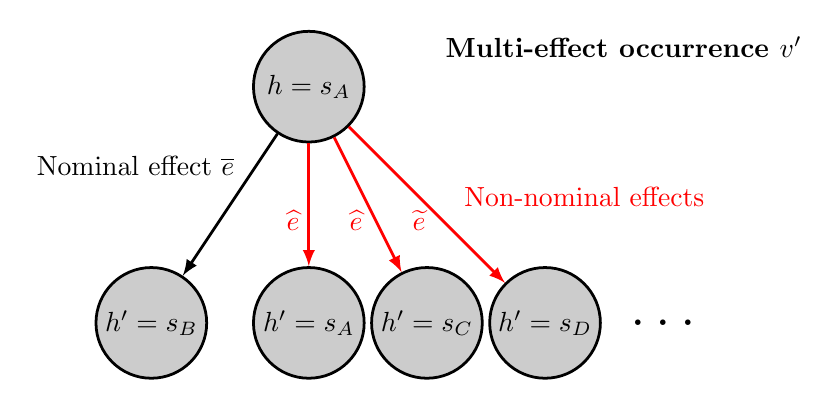
\begin{tikzpicture}
%states
\tikzstyle{vertex}=[circle,fill=black!20,draw=black, minimum size=40pt,line width=1pt,inner sep=0pt]
%1
\node[vertex] (hstate1) at (3,3) { \textbf{$h=s_A$}};
%2
\node[vertex] (hstate2) at (1,0) {$h'=s_B$};
\node[vertex] (hstate3) at (4.5,0) {$h'=s_C$};
\node[vertex] (hstate4) at (6,0) {$h'=s_D$};
\node (hstate5) at (7.5,0) {\huge $\ldots$};
\node[vertex] (hstate11) at (3,0) {$h'=s_A$};

\draw[->,>=latex,line width=1pt] (hstate1) -- (hstate2);
\draw[->,>=latex,color=red,line width=1pt] (hstate1) -- (hstate3);
\draw[->,>=latex,color=red,line width=1pt] (hstate1) -- (hstate4);
\draw[->,>=latex,color=red,line width=1pt] (hstate1) -- (hstate11);

\node (nominalEffect) at (0.8,2) {Nominal effect $\overline{e}$};
\node (nominalEffect) at (6.5,1.6) {{\color{red} Non-nominal effects}};

\node (nominalEffect) at (4.4,1.3) {{\color{red} $\widetilde{e}$}};
\node (nominalEffect) at (3.6,1.3) {{\color{red} $\widehat{e}$}};
\node (nominalEffect) at (2.8,1.3) {{\color{red} $\widehat{e}$}};

\node (occ) at (7,3.5) {\textbf{Multi-effect occurrence $v'$}};
\node (arrow) at (6,2.9) [rotate=230] { \huge$\rightsquigarrow$};
\end{tikzpicture}
\caption[Nominal and non-nominal effects]{Nominal effect and non-nominal effects of the occurrence $v'$ 
on the assessment $h \in \mathcal{S}$ which becomes $h' \in \mathcal{S}$.}
\label{multieffect}
\end{figure}

Non-nominal effects could also take place and correspond to 
assessment errors. Nevertheless for some occurrences only nominal effects are taken into account (\textit{i.e.} the observer does not foresees any human assessment error for those occurrences).
Occurrences with more than one possible effect for at least one possible assessment $h$ are called 
\textit{multi-effect} occurrences, and are illustrated in Figure
\ref{multieffect}. Formally if $v'$ 
and $h$ are such that $\exists (h_A',h_B') \in \mathcal{S}^2$ 
and $h_A' \neq h_B'$ for which $f_e(h,v',h_A')$ and $f_e(h,v',h_B')$ 
are defined, and $f_e(h,v',h_A') \neq f_e(h,v',h_B')$, 
$v'$ is a \textit{multi-effect} occurrence. 

The error model is completed 
once all non-nominal effects have been defined:
the logic table can be enhanced 
adding non-nominal effects for some occurrences. 
The way those non-nominal effects are described 
is  the same as for the nominal effects: 
by pairs (situation, behaviour) represented by columns of the logic table.
Referring to the example of the logic table given above (see Table \ref{trivialLogicTable}), the expert
knowledge could for instance assert that occurrence $v_C$  could possibly make the human believe that if the machine state is initially $s_A$ it finally changes to $s_B$. 
%has potentially a non-nominal effect on the human assessment (assessment error). 
This potential effect is described by column $4$ in Table \ref{trivialLogicTableEffect}. 
This new column does not replace the nominal case 
that is unaltered and still described by column $1$. 
For readability columns corresponding to non-nominal effects are written in red. Occurrence $v_C$ is thus a multi-effect occurrence. 
A logic table that includes assessment errors as Table \ref{trivialLogicTableEffect} is called an \textit{enhanced logic table}.
The expert knowledge may again enhance the error model,
stating that occurrence $v_A$ could also lead to the same kind of 
human assessment error (see column $5$).

Remember that effects $e$ concern the human assessment dynamics $h$, 
which is of course not observable: actual effects are thus not 
observable, as a result of $f_e(h,v',h')$. Effects can
however be sorted according to their plausibility,
as presented right now.

%Note that, replacing $s$ by $h$, those transitions 
%are the nominal effects of the possibilistic model that 
%will be defined later.

\subsection{Effect plausibility}
\label{effect_plausibility}
In this study nominal effects are considered 
as generally more plausible than the corresponding non-nominal ones 
\textit{i.e.} than the corresponding human assessment errors
starting from the same previous assessment $h$,
and under the same occurrence $v'$:
the human operator is thus assumed to know the machine logic 
and to have a quite good perception of the feedbacks.

Experts, after the enumeration of the potential non-nominal
effects, have also to sort all effects according to their plausibility, 
dividing them into categories: for instance, effects whose plausibility is normal 
$\overline{e}$ (shortly \textit{normal effects}), effects whose plausibility is less than normal but not unusual $\widehat{e}$ (shortly \textit{less than normal effects}), 
effects whose plausibility is unusual $\underline{e}$ (shortly \textit{unusual effects}), or even effects whose plausibility is very rare $\tilde{e}$ (shortly \textit{very rare effects}). 
The line ``effect'' is thus added to Table \ref{trivialLogicTableEffect} 
specifying effects plausibility. For instance, nominal effect described by
column $1$ is normal according to the expert ($\overline{e})$,
but nominal effect described by column $2$ is very rare ($\tilde{e}$).

%\renewcommand{\arraystretch}{1.5}
\begin{table}[t!]
  \centering
\resizebox{0.48\textwidth}{!}{
\begin{tabular}{!{\vrule width 2.2pt}c!{\vrule width 1.2pt}c!{\vrule width 1.2pt}c|c|c|c|c!{\vrule width 2.2pt}}
\specialrule{.22em}{.0em}{.0em}  	
columns		   &	&$1$&$2$&$3$& \color{red}{$4$}	& \color{red}{$5$}	\\ \specialrule{.22em}{.0em}{.0em}
\textbf{SITUATION} &		&   &	&	&			& 			\\ \specialrule{.22em}{.0em}{.0em}  
$v'$ 	& $v_A$ 	&$1$&	&	&	& \color{red}{$1$}	\\ \hline
		& $v_B$ 	&   &$1$&	& 	& 			\\ \hline
        & $v_C$ 	&$1$&   &   &\color{red}{$1$}&			\\ \specialrule{.1em}{.0em}{.0em}
$h$ 	& $s_A$   	&$1$&$1$&	&\color{red}{$1$} & 			\\ \hline
		& $s_B$ 	&   &	&$1$&	& \color{red}{$1$}	\\ \specialrule{.22em}{.0em}{.0em}
\textbf{BEHAVIOUR} &    &   &   &   &	&			\\ \specialrule{.22em}{.0em}{.0em}
$h'$ 	& $s_A$   	&	&   &	& 	& \color{red}{$1$}	\\ \hline
		& $s_B$ 	&	&$1$&	&\color{red}{$1$}&					\\ \specialrule{.22em}{.0em}{.0em}
\textbf{EFFECT} &   &$\overline{e}$&$\tilde{e}$&$\overline{e}$& $\color{red}{\widehat{e}}$&  \color{red}{$\underline{e}$}	\\ \specialrule{.22em}{.0em}{.0em}
\textbf{POSSIBILITY} &   & 1     & $\varepsilon$  	& 1 & \color{red}{$\lambda$} & \color{red}{$\delta$}	\\ \specialrule{.22em}{.0em}{.0em}
\end{tabular}%
}
\caption{Enhanced logic table of the logic table \ref{trivialLogicTable}:
occurrences $v_A$ and $v_C$ have both a non-nominal effect, described respectively by columns $5$ and $4$.
Each column represent a pair (situation, behaviour), and effect row represents the effect plausibility label.
Last row assigns a possibility degree to each effect (see section \ref{subsec:possibilisticModel}).
} \label{trivialLogicTableEffect}%
\end{table}%


We have made the assumption that for each assessment $h$, there always exists at least one occurrence $v'$ with a normal effect.
Thus, for each current human assessment $h$, it exists
one possible occurrence and next human assessment considered as normal \textit{i.e.}
\begin{equation}
\exists v', h' \mbox{ such that } f_e(h,v',h')=\overline{e}. 
\label{distribsNaturallyNormalized}
\end{equation}
This remark is essential and forms a rule imposed in practice when filling
the effect row of the enhanced enhanced logic table.
It means that for each human assessment, at least one next step of the 
human-machine interaction is normal. 
Moreover, this property suits
the possibilistic analysis model construction, 
as recalled section \ref{analysisModel}.

In the next section, the analysis model is defined from a given effect plausibility ranking, using a plausibility measure on the human-machine system dynamics:
more details about the chosen measure are given in section \ref{analysisModel}.
The last part of this section (\ref{workingAssumptions}) will derive the effect ranking from a set of expert rules, leading to a fully defined human-machine interaction model.  

Note that an effect is {\em normal} if its plausibility is considered as normal (by the expert, or the system designer).
Nominal effects and normal effects must not be confused 
(see Figure \ref{nominalNormal}): 
the words {\em normal, unusual} are used to define the plausibility 
of effects \textit{i.e.} to sort them, in order to
fully define the interaction model, 
as just explainded in this section \ref{effect_plausibility} 
and performed from general assumptions in section \ref{workingAssumptions}. 
On the other hand, effects are said {\em Nominal} if they represent a human assessment 
transition without error, \textit{i.e.}
a human assessment transition corresponding to the machine state 
transition (ideal human understanding). 
Thus, effects are said {\em non-nominal} 
if they represent assessment errors, and
are added to the logic table using expert knowledge.

\begin{figure}
        \centering
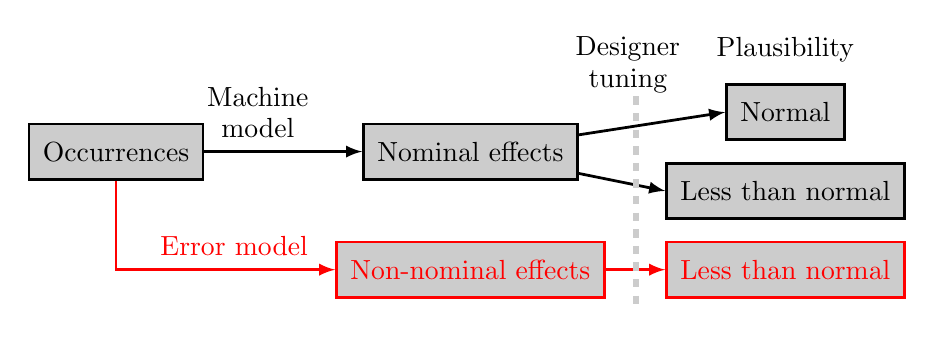
\begin{tikzpicture}
\tikzstyle{vertex}=[fill=black!20,draw=black, minimum size=20pt,line width=1pt,inner sep=5pt]
\tikzstyle{vertexRed}=[fill=black!20,draw=red, minimum size=20pt,line width=1pt,inner sep=5pt]

\node[vertex] (events) at (0,0) {Occurrences};
\node[vertex] (nominal) at (4.5,0) {Nominal effects};
\node[vertex] (normal) at (8.5,0.5) {Normal};
\node[vertex] (less1) at (8.5,-0.5) {Less than normal};

\node[vertexRed] (nonNominal) at (4.5,-1.5) {{\color{red}Non-nominal effects}};
\node[vertexRed] (less2) at (8.5,-1.5) {{\color{red}Less than normal}};

\draw[->,>=latex,line width=1pt] (events) -- (nominal);
\draw[->,>=latex,line width=1pt] (nominal) -- (normal.west);
\draw[->,>=latex,line width=1pt] (nominal) -- (less1.west);

\draw[->,>=latex,line width=1pt, color=red!] (events) |- (nonNominal);
\draw[->,>=latex,line width=1pt, color=red!] (nonNominal) -- (less2);

\node () at (1.8,0.7) {{Machine}};
\node () at (1.8,0.3) {{model}};

\node () at (1.5,-1.2) {{\color{red} Error model}};

\node () at (8.5,1.3) {{Plausibility}};

\node () at (6.5,1.3) {Designer};
\node () at (6.5,0.9) {tuning};

\draw[line width=2pt, color=black!20, dashed] (6.6,0.7) -- (6.6,-2);

\end{tikzpicture}
        \caption{Nominal effects, non-nominal ones defining the error model, and plausibility evaluation.}
        \label{nominalNormal}
\end{figure}


In the following section \ref{sec:traj} 
the human-machine interaction system dynamic is detailed.


\subsection{System dynamics: trajectories and exceptions}
\label{sec:traj}
After the manifestation of $m \geqslant 0$ occurrences, 
the sequence of machine states is called the $(m+1)$-length 
\textit{state trajectory} and is denoted by 
$\mathcal{S}_m = (s_0,s_1,\ldots,s_m)$.
This trajectory is considered as observable, as well as the $(m+1)$-length 
\textit{occurrence trajectory} $\mathcal{V}_m = (v_0,v_1, \ldots, v_m)$.
In other words the observer defined in introduction section \ref{intro} 
and Figure \ref{Observer}, thanks to their 
knowledge of the machine logic, is able to provide
% and the observation of the occurrences, 
%deduces the machine state.
%\textit{i.e.} 
$\forall 0 \leqslant t \leqslant m$, 
%defined as the variable containing
\begin{itemize} 
\item the occurrence at stage $t$, $v_t$ (e.g. selection, or automated state change),
\item and actual state of the machine $s_t$, deduced from the machine logic.
\end{itemize}
%These data all the observable data, \textit{i.e.} all data available for 

% Therefore the \textit{state trajectory} is part of the 
%\textit{occurrences trajectory}. 
%In fact, the occurrences trajectory 
%Note that, the the enhanced logic table 
%is exclusively dedicated to model the human assessments $h$ dynamics, 

However the actual \textit{effect trajectory} 
$(e_0,e_1,\ldots,e_m)$ and \textit{assessment trajectory} 
$(h_0,h_1,\ldots,h_m)$ are not observable. They may be estimated using 
the possibilistic analysis model described in section \ref{analysisModel}.
Remember that each occurrence may have many effects.
So a $(m+1)$-length occurrence trajectory corresponds 
to many possible $(m+1)$-length effect trajectories: 
$\forall 0 \leqslant t \leqslant m$, 
$e_t$ is an effect\footnote{Remember that effects are not observables.} of the occurrence $v_t$.
Each time a multi-effect occurrence is fired, several 
{\em assessment trajectories} are possible, one or more 
for each possible effect (see Figure \ref{multieffect}). The set of possible effects trajectories is denoted by $\mathcal{E}_m$ and the set of possible 
assessments trajectories $\mathcal{H}_m$.

In practice, possible effects and assessments trajectories 
are stored together in the form of 
\textit{non-observable trajectories}: 
$(e_0,h_0,e_1,h_1, \ldots, h_{m-1}, e_m, h_m)$ with 
$\forall 0 \leqslant t \leqslant m$, $e_t = f_e(h_{t-1},v_{t},h_t)$
if $f_e$ is defined for this triplet, 
and removing $h_{-1}$ for $t=0$.
The firing of a new occurrence $v_{m+1}$ updates 
the set of non-observable trajectories 
adding possible effects and assessments.
Each non-observable trajectory ending with 
$h \in \mathcal{S}$ at stage $m$, is completed with each pair 
$(f_e(h,v_{m+1},h'),h')$ such that $f_e(h,v_{m+1},h')$ is defined,
\textit{i.e.} stored in the enhanced logic table. 
% with affect all the assessment 
%trajectories (adding new possible effects), which subsequently evolve in time. 
Because several multi-effect occurrences may be fired the number of possible 
non-observable trajectories may increase significantly.

Initially the most plausible non-observable trajectory is the one that includes only 
nominal effects (\textit{i.e.} no assessment errors). 
%Indeed, occurrences effects of 
%this assessment trajectory lead to estimate that assessment $h$ is equal to the actual 
%state $s$. 
The corresponding assessment trajectory 
(removing effects from the non-observable trajectory) 
is called the {\em objective assessment trajectory} 
and is equal to the machine state trajectory. 
After the firing of an occurrence 
whose effects are all considered at the most as unusual 
in the actual situation, 
the objective assessment trajectory 
is no longer considered as normal. 
This situation is called an {\em exception} 
and the occurrence that led to the exception 
a {\em triggering occurrence}. 
Typical triggering occurrences are selections 
considered as erroneous in the particular context. 

Let us describe the mechanism and the behaviour
of the wanted analysis model which will be set up in section \ref{subsec:possibilisticModel}. 
If an exception is detected by the analysis model, 
the model itself verifies if there is a non-nominal effect 
(\textit{i.e.} an assessment error) in the past history that, 
if considered as the actual effect, 
could lead to a situation in which the firing of the triggering occurrence 
is not unusual, but instead normal. 
For instance the analysis models may verify 
if there is a human feedback misinterpretation 
that could explain a human selection otherwise considered as erroneous. 
This non-nominal effect is called \textit{exception explanation} 
and the assessment trajectory embedding this exception explanation 
is considered as the new most plausible one. 
The formerly most plausible assessment trajectory 
is no longer coherent with the actual observations of the system. 
Therefore, its plausibility is decreased. 
%For instance the first time an exception is detected the most plausible assessment trajectory is the {\em objective assessment trajectory}, this trajectory is no more coherent, and its plausibility is decreased.
On the other hand, if no exception explanation is found, 
the plausibility of the assessment trajectories remains unchanged.
The \textit{possibilistic Bayes rule}, 
also presented in the section \ref{analysisModel},
formally defines how to implement these concepts. 

The following section \ref{workingAssumptions} 
presents the expert rules chosen 
to complete the human-machine interaction model:
these assumptions about effects are
used in applications presented in last sections 
\ref{sec:mockup} and \ref{sec:flightSim}.


\subsection{Working assumptions}
\label{workingAssumptions}

In order to define in practice non-nominal effects 
modelling human operator assessment errors,
as well as their plausibility, two methods are possible: 
designing them one by one \textit{by hand} with the help of experts of the domain, 
or deriving them \textit{mechanically} from a limited number of general assumptions formulated by the experts.
Nevertheless a mixed approach is also possible: 
for instance designers could start with the \textit{mechanical} assumption-based method 
and successively suppress or add \textit{by hand} some non-nominal effects, 
or even rank \textit{by hand} the plausibility of some effects.

Hereafter some assumptions for the mechanical approach about possible effects and their plausibilities are defined. 
%The modelling process (starting from the definition of these assumptions) 
%is detailed hereafter. 
Defining a generic set of assumptions is out of the scope 
of this work. Note that these rules have been defined by experts for
the experiment presented in section \ref{sec:flightSim}, and may be unsuitable for other applications. 
They are defined here to set an example of interaction model 
(including the ranking of effects), before the building of the possibilistic analysis model.

Here is the list of the chosen working assumptions:
%{\bf Structure of the model}\\
%\begin{itemize}
%\item the human knowledge of the machine behaviour is correct
%\end{itemize}
%This assumption implies that the human is sufficiently trained to use the machine and knows its behaviour.\\
%
%{\bf occurrence effects possibility}\\
\begin{itemize}
\item the human knowledge of the machine behaviour is correct;
\item the human should perceive feedbacks, but she/he can possibly miss them;
\item the human knowledge of the initial state is uncertain, but is likely to coincide with the real one;
\item selections that do not change the machine state are considered as {\em slips}, \textit{i.e.} unmeant selections;
\item the missing of a feedback is more likely to happen than a slip or a mistake:
a \textit{mistake} is a selection or a lack of selection 
defined as erroneous by the system designer.
\item the missing of $n<n_{max}$ feedbacks is more likely to happen than missing $n+1$ feedbacks, or a slip.
\end{itemize}
The first assumption implies that the human is sufficiently 
trained to use the machine and knows its behaviour: 
nominal effects are then generally considered
as more plausible than the corresponding non-nominal ones.
as previously announced.

According to the next two assumptions, the interaction model takes 
into account two multi-effect occurrences. The first one 
is the feedback sending: feedbacks should be perceived 
(nominal effect) but could go unseen (non-nominal effect). 
The second one is the initial human appreciation of the 
machine state: the initial assessment should be correct 
(nominal effect), but could be wrong (non-nominal effect).

The fourth assumption means that selections which do not change 
the machine state are not voluntary. 
The last assumption states that the more feedbacks
are lost, the less the situation is plausible.

% In this model only occurrences having at least a normal 
%effect are modelled as a multi-effect occurrence, but the same can be done in principle with occurrences 
%that have no normal effect.

For this interaction model, the following occurrences
and corresponding effects are thus used:
\begin{itemize}
\item the execution of selections which have one nominal effect; depending on the current assessment they are classified as normal selections, or as slips/mistakes which are unusual;
%with one effect (nominal);
%\item the execution of a slip, 
\item  an {\em automated state change}
with two possible effects: the reception and well interpretation of the relevant feedback (nominal), which is normal, 
and the loss of the feedback (non-nominal), which is not normal but more likely to happen than an unusual effect; 
\item  the state initialization with two possible effects: correct initialization (nominal), which is normal, and wrong initialization (non-nominal), which is unusual. 
\end{itemize}

\begin{figure} \centering
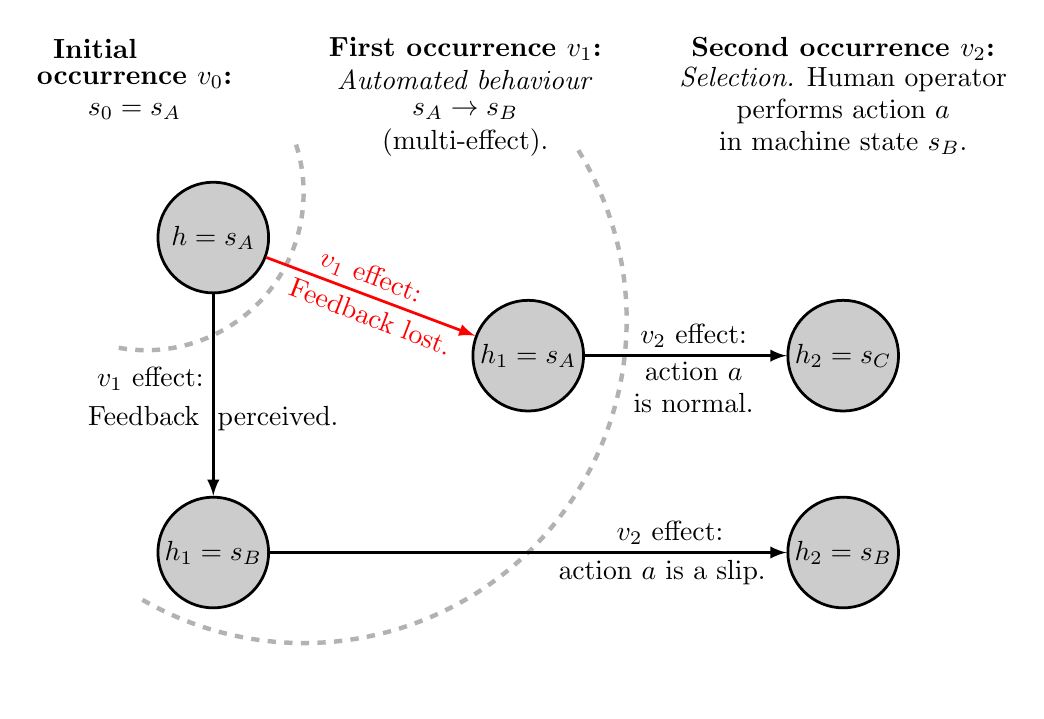
\begin{tikzpicture}
%states
\draw[ultra thick,draw=black!30, dashed] (2.1,-1.6) arc (-120:33:4.1cm);
\draw[ultra thick,draw=black!30, dashed] (1.8,1.6) arc (-100:20:2cm);

\tikzstyle{vertex}=[circle,fill=black!20,draw=black, minimum size=40pt,line width=1pt,inner sep=0pt]
%1
\node[vertex] (hstate1) at (3,3) { \textbf{$h=s_A$}};
%2
\node[vertex] (hstatep1) at (7,1.5) {$h_1=s_A$};
\node[vertex] (hstatep2) at (3,-1) {$h_1=s_B$};
%3
\node[vertex] (hstatepp3) at (11,-1) {$h_2=s_B$};
\node[vertex] (hstatepp4) at (11,1.5) {$h_2=s_C$};

\draw[->,>=latex,line width=1pt,color=red] (hstate1) -- (hstatep1);
\draw[->,>=latex,line width=1pt] (hstate1) -- (hstatep2);
\draw[->,>=latex,line width=1pt] (hstatep1) -- (hstatepp4);
\draw[->,>=latex,line width=1pt] (hstatep2) -- (hstatepp3);

\node (occ1) at (1.5,5.4) {\textbf{Initial}};
\node (occ1) at (2,5) {\textbf{occurrence $v_0$:}};
\node (occ1) at (2,4.6) {$s_0=s_A$};

\node (occ1) at (6.2,5.4) {\textbf{First occurrence $v_1$:}};
\node (occ1) at (6.2,5) {\textit{Automated behaviour}};
\node (occ1) at (6.2,4.6) {$s_A \rightarrow s_B$};
\node (occ1) at (6.2,4.2) {(multi-effect).};
\node (arrow) at (5.9,3.5) [rotate=240] { \Huge$\rightsquigarrow$};

\node (nominalEffect1) at (2.2,1.2) {$v_1$ effect: };
\node (nominalEffect11) at (3,0.7) {Feedback \ perceived.};
\node (Effect1) at (5,2.5) [rotate=339] {{\color{red} $v_1$ effect:}};
\node (Effect11) at (5,2) [rotate=339] {{\color{red} Feedback lost.}};

\node (occ2) at (11,5.4) {\textbf{Second occurrence $v_2$:}};
\node (occ2) at (11,5) {\textit{Selection.} Human operator};
\node (occ2) at (11,4.6) {performs action $a$};
\node (occ2) at (11,4.2) {in machine state $s_B$.};
\node (arrow) at (11,3.5) [rotate=240] { \Huge$\rightsquigarrow$};

\node (nominalEffect1) at (8.8,-0.75) {$v_2$ effect: };
\node (nominalEffect11) at (8.7,-1.25) {action $a$ is a slip.};
\node (Effect1) at (9.1,1.75) {$v_2$ effect:};
\node (Effect11) at (9.1,1.3) {action $a$};
\node (Effect111) at (9.1,0.9) {is normal.};

\end{tikzpicture}
\caption{Loss of feedback as an exception explanation.}
 \label{explaination}
\end{figure}

The interaction model is so fully defined.
The analysis model detailed in the next section is based on the Qualitative Possibility Theory (see Section \ref{posspres}) 
providing a formal way to sort effects according to their plausibility. 
Starting from a human-machine interaction model, built as presented in the current section, 
the analysis model leads to a possibilistic estimation of the human assessment at each step of the process.

Before detailing the analysis model let us show with an example the desired comportment of the model for an automated state change followed by an action that is a slip in the actual state of the machine (see Figure \ref{explaination}).

Let us start with the automated state change with machine initial state $s_A \in \mathcal{S}$  
and final state $s_B \in \mathcal{S}$. 
The correct reception of the relevant feedback 
has to be considered as the most plausible effect. 
The objective assessment trajectory ($h_0=s_A$, $h_1=s_B$) 
has to be normal and so the most plausible one. 
The second trajectory ($h_0=s_A$, $h_1=s_A$) 
corresponds to the loss of feedback 
and it has to be less than normal but more than unusual.

Later on the human performs a selection (action $a$) 
that does not modify the machine state. 
This selection is a slip in the actual state of the machine: $s_B$. 
Therefore it is a slip also for a human operator for which $h_1=s_B$. 
The objective assessment trajectory becomes ($h_0=s_A$, $h_1=s_B$, $h_2=s_B$), 
and its plausibility should be reduced to that of a slip (unusual).

If the human assessment has not been updated in step $1$ due to a loss of feedback (second trajectory) 
the assessment is still $h_1=s_A$. 
Suppose that in this machine state $s_A$ action $a$ is totally normal. 
The second trajectory becomes ($h_0=s_A$, $h_1=s_A$, $h_2=s_C$) and its plausibility should remain unchanged (less than normal but more than unusual).

An exception should be detected and the analysis model should identify the exception explanation in the loss of the 
relevant feedback.

\section{Human assessment estimation, error detection and diagnostic}
\label{analysisModel}
Possibility Theory is well suited to encode
qualitative expert knowledge such as 
the working assumptions presented in the previous section.
This section begins with a short presentation 
of this theory. Later on the first step of
the possibilistic analysis model is presented: 
starting from the interaction model, 
natural language knowledge is expressed in terms 
of possibility degrees: basically, 
what was ``plausible'' becomes ``possible'', 
what was ``less normal'' is defined as ``less possible'', 
what was ``unusual'' becomes ``far less possible'', 
and what was ``very rare'' becomes ``almost impossible''.
This section ends with formal computations 
leading to successive human assessment 
estimations, the error assessment detection 
and the exception explanation.
%Possibility theory \cite{Dubois07} is part of Uncertainty Theories 
%and is devoted to the handling of incomplete information. 
%It can capture partial ignorance about the uncertainty model. 

Here the problem deals with uncertainty 
related to the effects of each occurrence,
\textit{i.e.} the human assessment transitions: 
in situations where no wide enough experiments dataset are available, 
the corresponding uncertainty cannot be modelled precisely 
with frequencies leading to transition probabilities. 
Possibility Theory allows the definition of a model 
using only the available information about the system, 
which is however enough rich to build a useful model. 
%More specifically, 
%our model is based on the Qualitative Possibility Theory.

%This theory encodes uncertainty through fuzzy measures, 
%fully specified by \emph{possibility distributions}:
%a possibility distribution is a mapping $\pi$ 
%from a set of states of the world $\mathcal{X}$ 
%to a totally ordered scale $\mathcal{L}$, 
%whose lowest element is denoted by $0$, 
%and highest one by $1$. 
%The function $\pi$ represents knowledge 
%(about the actual state of the world $x \in \mathcal{X}$) 
%distinguishing what is plausible from what is less plausible.
%It represents a flexible restriction on what the actual state of affairs is, 
%with the following conventions:
%\begin{itemize}
%   \item 
%An impossible state of the world $x \in \mathcal{X}$ 
%has a possibility degree equal to $0$ 
%\textit{i.e.} $\pi(x)=0$ means that state $x$ is impossible; %means that state {\em s} is rejected as impossible
%moreover, for a couple $(x,x') \in \mathcal{X}^2$, $\pi(x)<\pi(x')$ 
%encodes that $x$ is less plausible than $x'$;
%\item 
%finally possibility degree of $x \in \mathcal{X}$ is maximal, 
%\textit{i.e.} $\pi(x)=1$, if the state $x$ is part of the most possible 
%(plausible, unsurprising, normal, \ldots) states of the world.
%\end{itemize}
%If the state space $\mathcal{X}$ is exhaustive, at least one of its elements should be the actual world, so that at least one 
%state is totally possible: 
%It leads to the possibilistic normalization $\max_{x \in \mathcal{X}} \pi(x) = 1$. 

%While a probability distribution provides 
%a quantitative measure of occurrence of an event 
%(frequencies $\in [0,1]$), 
%a possibility one only sorts these events 
%using the qualitative scale $\mathcal{L}$.
%Possibility Theory and Probability Theory 
%share some similar properties: 
%for example, a possibility distribution
%looks like a probability distribution 
%(a function from $\mathcal{X}$ 
%to a structured space: $\mathcal{L}$ or $[0,1]$). 
%Moreover a possibilistic counterpart 
%of the Bayes Rule \cite{Dubois199023} is available: 
%introducing a set of possible observations $y \in \mathcal{Y}$, 
%and an observation possibility distribution knowing each state of the world, 
%$(x,y) \mapsto \pi \paren{ y \sachant x }$, 
%a posterior possibility distribution can be deduced 
%from a prior possibility distribution $x \mapsto \pi(x)$ 
%and the actual observation $y_{obs} \in \mathcal{Y}$. 
%This posterior possibility distribution over the state of the word is
%\begin{equation}
%\pi \paren{x \sachant y_{obs}} = \left \{ \begin{array}{ccc}
%1 & \mbox{ if } x \in \displaystyle \operatorname*{argmax}_{x \in \mathcal{X}} \pi \paren{y_{obs}, x } \\
%\pi \paren{y_{obs}, x } & \mbox{otherwise,}
%\end{array} \right.
%\label{bayesRule}
%\end{equation}
%where $\pi \paren{y_{obs}, x }=\min \set{ \pi \paren{y_{obs} \sachant x }, \pi(x) }$.
%It defines the possibilistic Bayes rule.

\subsection{Possibilistic analysis model}
\label{subsec:possibilisticModel}
In order to perform the possibilistic analysis 
the interaction model has to be fully defined, 
\textit{i.e.} all the effects 
have to be defined and sorted according to their plausibility. 
The effect ranking can be encoded defining an appropriate qualitative 
scale $\mathcal{L}$ and assigning possibility degrees from
this scale to the effects. 
The example of table \ref{trivialLogicTableEffect}
defines the qualitative scale $\mathcal{L}$ as 
$\set{ 0, \varepsilon, \delta, \lambda, 1 }$
with $0 < \varepsilon < \delta < \lambda < 1 $, 
and assigns possibility degree $1$ to normal effects, 
$\pi(\overline{e})=1$, 
degree $\lambda$ to less normal effects, 
$\pi(\widehat{e}) = \lambda$, 
degree $\delta$ to unusual effects 
$\pi(\underline{e})=\delta$, 
and degree $\varepsilon$ to very rare effects, 
$\pi(\tilde{e})=\varepsilon$.
Of course, if a transition is impossible, \textit{i.e.} if function $f_e$ is not defined,
corresponding possibility degree is $0$. 
This last modelling step leads to the full definition 
of a possibilistic hidden Markov process whose states
are the successive human assessments, sound framework for human assessment estimation.

The interaction model used in this work has
been set up in section \ref{workingAssumptions}, 
providing definition of occurrence effects 
and the ranking of those effects.  
The possibility degrees have still to be assigned
to them.
Occurrence effects possibility degrees are  
in the qualitative scale $\mathcal{L}=\set{0,\varepsilon,\lambda,1}$ 
with $0<\varepsilon<\lambda<1$.
The following notations defining classes of effects are useful 
to assign possibility degrees:
%Machine state is represented by variable $s \in \mathcal{S}$, estimated human assessment 
%by variable $h \in \mathcal{S}$, and human operator's selection effect by $e_{sel}$. 
%We assume that human does not execute useless selections on purpose:
%if $e_{sel}$ is useless given $h$ then $\pi \paren{ e_{sel} \sachant h } = \pi(e_s) = \varepsilon$.
%Naturally, $\pi \paren{ e_{sel} \sachant h } = 1$ otherwise.
\begin{itemize}
\item $e_{0c} \doteq$ the correct initialization -- nominal effect of an ``initialization'' occurrence,\\ $\pi(e_{0c})=1$;
\item $e_{0w} \doteq$ a wrong initialization -- non-nominal effect of an ``initialization'' occurrence,\\ $\pi(e_{0w})=\varepsilon$;
\item $e_f \doteq$ the correct reception of a feedback -- nominal effect of an ``automated behaviour" occurrence: $\pi(e_f)=1$;
\item $e_l \doteq$ a missed feedback -- non-nominal effect of an ``automated behaviour" occurrence: $\pi(e_l)=\lambda$;
%\item $e_n \doteq$ a generic normal selection effect, $\pi(e_{sel})=1$; ??? $e_n$ ??
\item $e_{n} \doteq$ a generic occurrence effect considered as normal, other than $e_{0c}$ and $e_f$ (for instance a normal selection): $\pi(e_{n})=1$;
\item $e_s \doteq$ the arising of a slip -- nominal effect of a selection occurrence, $\pi(e_s) = \varepsilon$;
\item $e_m \doteq$ a mistake -- nominal effect of a selection or ``absence of selection" occurrence, $\pi(e_m) = \varepsilon$.
\end{itemize}
%  
%\begin{description}
%\item  $e_f \doteq$ the correct reception of a feedback (nominal effect)
%\item  $e_l \doteq$ a missed feedback (non-nominal effect)
%\item  $e_s \doteq$ the arising of a slip or a mistake (nominal effect)
%\item  $e_{0c} \doteq$ the correct initialization (nominal effect)
%\item  $e_{0w} \doteq$ a wrong initialization (non-nominal effect)
%\item  $e_{normal} \doteq$ a generic occurrence effect considered as normal
%\item  $e_{unusual} \doteq$ a generic occurrence effect considered as unusual
%\item  $e_{sel} \doteq$ a generic selection effect\\
%\end{description}
% assessment trajectories of interest and their possibility degrees. 
%The set of constraints (needed for this qualitative approach) is build on assumptions 
%concerning the structure of the model, the 
%Event effects possibility degree,  and the 
%assessment trajectories possibility. %We have already presented some of those assumptions  

%We assume that human's knowledge of the machine behaviour is correct. This assumption 
%implies that human is sufficiently trained to use the machine and knows its behaviour.
%It may be later relaxed so as to enrich the model with the most common human errors.

The human assessment of the initial state is uncertain, 
but is likely to coincide with the real one, 
\textit{i.e.} a correct initialization is more plausible 
than a wrong one: $1=\pi(e_{0c})>\pi(e_{0w})=\varepsilon$.
Moreover, the good reception of a feedback is more plausible 
than a loss of one of them, 
which is more likely to happen than a slip or a mistake: 
$\pi(e_f) = 1 > \pi(e_l) = \lambda > \pi(e_s) = \pi(e_m) = \varepsilon$.

Before starting the human assessment estimation, 
it is important to understand the link between 
possibility degrees of effects, 
and possibilistic system dynamics. 
An effect encodes the manifestation of an occurrence $v'$
and the transition from current human assessment $h \in \mathcal{S}$ 
to the next one $h' \in \mathcal{S}$: 
an effect is then plausible 
when occurrence $v'$ and assessment $h'$ are plausible 
knowing previous one $h$. 
That leads to the following equation 
defining the joint possibility distribution 
over next assessment and occurrence:
\begin{equation}
\pi \paren{ v', h' \sachant h } = \pi \paren{ f_e \paren{ h,v',h' } }
\label{EAO}
\end{equation}
\textit{i.e.} the possibility degree of the effect of an occurrence $v'$ 
is the joint possibility degree of the this occurrence ($v'$) 
and the next assessment ($h'$) associated with the effect, 
knowing current assessment ($h$).
For the initialization occurrence (beginning of the human-machine interaction), 
as no previous assessment is available, 
equation \ref{EAO} becomes simply:
$\pi \paren{ v_0, h_0} = \pi \paren{ f_e \paren{ v_0,h_0 } }.$
Note that initialization occurrence is artificially added to define initial uncertainty: 
it is thus considered as a totally normal occurrence: $\pi(v_0) = 1$.
Then $ \pi \paren{ v_0, h_0} = \min \set{ \pi(v_0), \pi \paren{ h_0 \sachant v_0 } } = \pi \paren{ h_0 \sachant v_0 }$, \textit{i.e.}
\begin{equation}
\label{EAOinit} \pi \paren{ h_0 \sachant v_0} = \pi \paren{ f_e \paren{ v_0,h_0 } }.
\end{equation}

Recall that the possibility degree $0$ is of course assigned 
to each triplets $(h,v',h')$ for which 
$f_e$ is not defined: 
no such effects have been declared possible by experts.

As explained around equation \ref{distribsNaturallyNormalized} 
for each assessment $h$, 
there exists an occurrence $v'$ 
and a human assessment $h'$
entirely possible:
there is always a couple $(v',h')$ 
such as $\pi \paren{ v', h' \sachant h } = 1$.
Thus $\pi \paren{ v', h' \sachant h }$ 
defines actually a joint possibility distribution,
as possibilistic normalization is naturally ensured.

\subsection{Human assessment estimation}
Initial possibility distribution over human assessment $h$ 
is denoted by $\pi_0 \paren{ h } = \pi \paren{ h_0 = h \sachant v_0 }$
which depends on initial occurrence $v_0$ 
defining initial machine state $s_0$.
It encodes the initial estimation 
of the human assessment about the machine state,
using assumptions of the interaction model: 
knowing the initial machine state, 
as part of data available for the observer, 
a positive possibility degree is assigned 
to each potential human operator initial assessment 
of the machine state,
using equation \ref{EAOinit}.
%As show just below for the \textit{transition function}, $\pi_0$ can be computed
%using Bayes rule \ref{bayesRule} and equality \ref{EAO} which becomes 
%$\pi \paren{ f_e(v,h) } = \pi(v_0=v,h_0=h)$ for initialization (no previous assessment).

Given occurrence $v_{t+1}$, the possibilistic dynamics of human belief (assessment), 
\textit{i.e.} the possibility degree of each assessment transition, 
is summed up in the transition function 
$(h,h') \mapsto T_{t+1} \paren{h,h'} = \pi \paren{ h_{t+1} =h' \sachant h_t = h, v_{t+1}} $.
\begin{Def}[Transition function]
As $\pi \paren{ v_{t+1},h' \sachant h }$ is given by the interaction model,
using equation \ref{EAO}, and as $v_{t+1}$ is known, $T_{t+1}$ is 
computed with normalization \\ $T_{t+1} \paren{h, h'} =$  
$\left \{ \begin{array}{ccc}
1 \mbox{ if } h' \in \displaystyle \operatorname*{argmax}_{h' \in \mathcal{S}}  \pi \paren{v_{t+1},h' \sachant h }  \\
\pi \paren{v_{t+1},h' \sachant h } \mbox{ otherwise, }
\end{array} \right .$ 
which comes directly from possibilistic conditionning \ref{def_cond}.
\label{transFunc}
\end{Def}
The occurrences sequence $(v_t)_{t \in \mathbb{N}}$
only concerns actual facts (\textit{e.g.} 
human operator selection, automated behaviour, \ldots) 
that are available (fully observable):
$T_t$ is then in fact a transition possibility distribution 
of the non-stationary possibilistic Markov Chain 
$(h_t)_{t \in \mathbb{N}} \in \mathcal{S}^{\mathbb{N}}$ 
with initial possibility distribution $\pi_0$.
This formalism is the same as the one used in the previous chapter
for planning under uncertainty \cite{Drougard13}. 
Here, unlike in planning problems,
no action has to be chosen
in this framework: 
however hidden state (here human assessment) 
is inferred in the same way.
As successive human assessments constitute states of the Markov process, 
and are not directly observable, 
the analysis model is in fact summed up 
in a possibilistic hidden Markov process 
illustrated by Figure \ref{diag}.
%$T_{t+1} \paren{ h' \sachant h} =  \pi \paren{ h_{t+1} = h' \sachant h_t = h, v_{t+1} = v } $
%\begin{equation}
%\label{transComp}
% = \max_{e \in \mathcal{E}} \min \set{ \pi_{t+1} \paren{ h' \sachant h, e}, \pi_{t+1} \paren{ e \sachant v} }.
%\end{equation}
%\[ = \displaystyle \max_{e \in \mathcal{E}} \min \left \{ \begin{array}{c}
%\pi \paren{ h_{t+1} =h' \sachant h_t = h, e_t = e}, \\
% \pi \paren{ e_t = e \sachant v_t = v} 
%\end{array}
%\right \}
%\]

At occurrence step $t$, 
the \emph{possibilistic estimation of the human assessment} 
is defined by the following possibility distribution:
\begin{Def}[Possibilistic estimation of the human assessment]
\begin{equation}
\label{estimH}
\pi_{t} \paren{ h } = \pi \paren{ h = h_t \sachant v_0, \ldots, v_t  }
\end{equation}
\end{Def}

As illustrated in Figure \ref{diag}, 
some occurrences (as selections), depends on the previous belief (assessment) of the human
operator \textit{i.e.} possibility degree of occurrence $v_{t+1}$ depends on $h_t$,
and this dependence is defined bu the observation function 
$(h,v') \mapsto O \paren{h,v'} = \pi \paren{ v_{t+1}=v' \sachant h_t=h }$:
this information is used to update the current estimation $\pi_t$.

\begin{figure}\centering
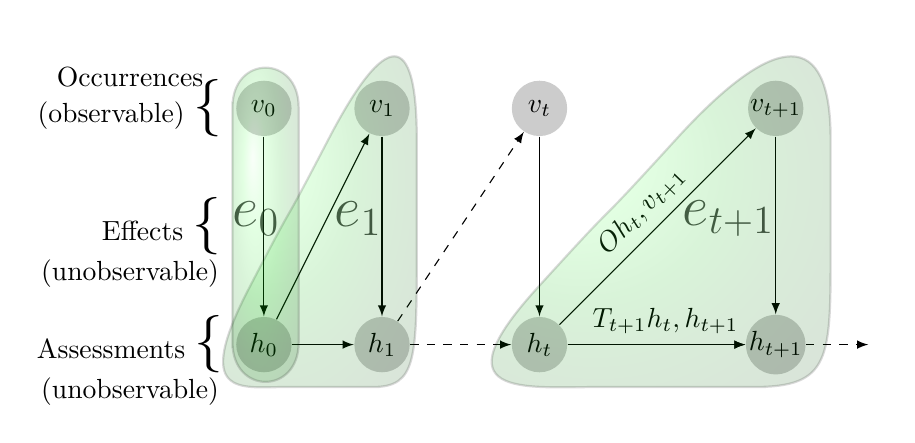
\begin{tikzpicture}%[scale=0.8,transform shape]
%TIME
%\node [font=\huge] (statet) at (3.8,1) {$t$};
%\node [font=\huge] (statetplus1) at (8.9,1) {$t+1$};
%%%%%%%%%%%%%%%%%%%%%%%%%%%%%%%%%%%%%%%%%%%%%%%%%%%%%%%%%%%%%%%%%%%%%%%%
%states
\tikzstyle{vertex}=[circle,fill=black!20,minimum size=20pt,inner sep=0pt]
\node (Oc) at (1.3,3.4) {Occurrences};
\node (V) at (1.3,3) {(observable) \huge $\{$};
%\node (V) at (1.5,1) {effects \huge $\{$};
\node (H) at (1.3,0) {Assessments \huge $\{$};
\node (H) at (1.3,-0.6) {(unobservable)};

\node (E) at (1.7,1.5) {Effects \huge $\{$};
\node (E2) at (1.3,0.9) {(unobservable)};

%1
\node[vertex] (state1) at (3,3) {$v_0$};
%\node[vertex] (state11) at (2.5,1) {$e_0$};
\node[vertex] (state111) at (3,0) {$h_0$};
%2
\node[vertex] (state2) at (4.5,3) {$v_1$};
%\node[vertex] (state22) at (4,1) {$e_1$};
\node[vertex] (state222) at (4.5,0) {$h_1$};

\node[vertex] (state3) at (6.5,3) {$v_t$};
%\node[vertex] (state33) at (6,1) {$e_t$};
\node[vertex] (state333) at (6.5,0) {$h_t$};

\node (T) at (8.1,0.3) {$T_{t+1} \paren{h_t,h_{t+1}}$};
\node (H) at (7.8,1.7) [rotate=46] {$O \paren{h_t,v_{t+1}}$};

\node[vertex] (state4) at (9.5,3) {$v_{t+1}$};
%\node[vertex] (state44) at (8,1) {$e_{t+1}$};
\node[vertex] (state444) at (9.5,0) {$h_{t+1}$};


\node (state23) at (10.5,3) {$\hdots$};

%3
\node (state5) at (10.8,2) {};
\node (state55) at (10.8,1) {};
\node (state555) at (10.8,0) {};

\node (e0) at (2.9,1.6) [color=black!70] {\huge $e_0$};
\node (e1) at (4.2,1.6) [color=black!70] {\huge $e_1$};
\node (et) at (8.9,1.6) [color=black!70] {\huge $e_{t+1}$};

%SV
% arrows sv->sv
%1->2
\draw[->,>=latex] (state1) -- (state111);
\draw[->,>=latex] (state111) -- (state2);
\draw[->,>=latex] (state111) -- (state222);
%\draw[->,>=latex] (state111) -- (state11);
%\draw[->,>=latex] (state1) -- (state11);


\draw[->,>=latex] (state2) -- (state222);
\draw[->,>=latex,dashed] (state222) -- (state3);
\draw[->,>=latex,dashed] (state222) -- (state333);
%\draw[->,>=latex] (state2) -- (state22);
%\draw[->,>=latex] (state222) -- (state22);
%\draw[->,>=latex] (state111) -- (state22);

\draw[->,>=latex] (state3) -- (state333);
\draw[->,>=latex] (state333) -- (state444);
\draw[->,>=latex] (state333) -- (state4);

%\draw[->,>=latex] (state333) -- (state33);
%\draw[->,>=latex] (state3) -- (state33);
%\draw[->,>=latex,dashed] (state222) -- (state33);
\draw[->,>=latex] (state333) -- (state444);
\draw[->,>=latex] (state4) -- (state444);
\draw[->,>=latex,dashed] (state444) -- (state555);

%\draw[->,>=latex] (state444) -- (state44);
%\draw[->,>=latex] (state4) -- (state44);
%\draw[->,>=latex] (state333) -- (state44);

\draw [scale=0.7,xscale=1.4, ball color=green,opacity=0.15,xshift=40,yshift=35,thick=5pt]
 (9,2.5)..controls +(0,2) and +(1.3,2) ..(7,2.5) % angle haut
 ..controls +(-1.3,-2) and +(1.3,2) ..(5.2,-0.2) % ligne gauche inclinee
 ..controls +(-1.3,-2) and +(-1,0).. (6,-2) % angle inferieur gauche
 ..controls +(-1,0) and +(1,0).. (8,-2)
 ..controls +(1,0) and +(0,-2).. (9,0.5) % angle inferieur droit
 ..controls +(0,1) and +(0,-1).. (9,2.5); % arc 4

\draw [scale=0.7,xscale=0.8, ball color=green,opacity=0.15,xshift=-5,yshift=35,thick=5pt]
 (9,2.5)..controls +(0,2) and +(1.3,2) ..(7,2.5) % angle haut
 ..controls +(-1.3,-2) and +(1.3,2) ..(5.2,-0.2) % ligne gauche inclinee
 ..controls +(-1.3,-2) and +(-1,0).. (6,-2) % angle inferieur gauche
 ..controls +(-1,0) and +(1,0).. (8,-2)
 ..controls +(1,0) and +(0,-2).. (9,0.5) % angle inferieur droit
 ..controls +(0,1) and +(0,-1).. (9,2.5); % arc 4


\draw [scale=0.7,xscale=0.8,yscale=0.95, ball color=green,opacity=0.15,xshift=-67,yshift=58,thick=5pt]
 (8.5,2.5)..controls +(0,1) and +(0,1) ..(7,2.5) % angle haut
 ..controls +(0,1) and +(0,-1) ..(7,-2) 
 ..controls +(0,-1) and +(0,-1).. (8.5,-2) % angle inferieur droit
 ..controls +(0,1) and +(0,-1).. (8.5,2.5); % arc 4

\end{tikzpicture}
\caption[Dynamic Bayesian Network of the $\pi$-HMP defining the analysis model.]{Dynamic Bayesian Network of the problem: relations between occurrences ($v_t$), and corresponding effects ($e_t$) on assessments evolution ($h_t$).}
\label{diag}
\end{figure}

\begin{Def}[Observation function]
As $\pi \paren{ v_{t+1},h' \sachant h }$ is given by equation \ref{EAO}, 
observation function is given by marginalization
$O \paren{h,v_{t+1}} = \max_{h' \in \mathcal{S}} \pi \paren{ v_{t+1},h' \sachant h }$
\label{obsFunc}
\end{Def}

The set of  assessments $h$ such that $\pi_{t} \paren{ h } = 1$ 
is denoted by $H_t^*$
(human assessments of the machine state that are totally possible). 
At step $t$ the next occurrence $v_{t+1}$ 
can contradict estimation of the assessment: 
an exception arises when the possibility degree of this occurrence $v_{t+1}$ 
knowing one of the most plausible $ h \in H_t^*$ 
is less than the same possibility degree 
knowing another human assessment 
$\tilde{h} \notin H_t^*$, $O (h, v_{t+1}) \leqslant O (\tilde{h}, v_{t+1})$, 
and less than current estimation of the latter 
$O (h, v_{t+1}) \leqslant \pi_t (\tilde{h})$. 
More generally, information given by next occurrence $v_{t+1}$ 
is used to update estimation, using next theorem. 
\begin{theorem} 
\label{thmUpdate}
Human assessment estimation update,
$\pi_{t}' \paren{h} = \pi \paren{ h_t = h \sachant v_0,v_1, \ldots, v_{t+1} }$,
can be computed as follow: 

$\pi_{t}' \paren{h} $
\begin{equation}
= \left \{ \begin{array}{ccc}
1 \hspace{0.5cm} \mbox{ if }  h \in \displaystyle \operatorname*{argmax}_{\mathcal{S}} \min \set{ O(h,v_{t+1}), \pi_t \paren{ h } }, \\
\hspace{-1cm} \min  \set{ O(h,v_{t+1}), \pi_t \paren{h}} \hspace{0.5cm} \mbox{ otherwise.}  
\end{array} \right .
\label{bayesUpdate}
\end{equation}
This equation does not modify assessment estimation 
($\pi_t \equiv \pi_t'$) 
if the following sufficient condition holds: 
$\forall h \in H_t^*$, $O \paren{ h, v_{t+1} } = 1$ 
and $\forall h \notin H_t^*$, $\pi_t \paren{ h } \leqslant O \paren{ h, v_{t+1}}$.
\end{theorem}
\begin{proof}
Qualitative possibilistic conditionning \ref{def_cond} 
provides equation \ref{bayesUpdate}, observation function
playing the role of $\pi \paren{ y_{obs} \sachant x }$,
occurrence $v_{t+1}$ the observation role, and 
assessment $h$ the role of the state.
Now, if $\forall h \in H_t^*$, $O \paren{ h, v_{t+1}} = 1$, 
as $\pi_t(h)=1$, the first case occurs
and $\pi_t' \paren{h} = \pi_t \paren{h} = 1$. 
The same equation holds $\forall h \notin H_t^*$: 
as $\pi_t \paren{ h } < 1$, 
the second case (``otherwise") occurs, 
and as $\pi_t \paren{ h } \leqslant O \paren{ h, v_{t+1}} $,
$\pi_t' (h) = \min \set{ \pi_t \paren{ h } , O \paren{ h, v_{t+1}}} = \pi_t (h)$.
\end{proof}

It is now possible to formally define an exception: 
\textbf{an exception is detected at step $t+1$ 
when update \ref{bayesUpdate} 
makes the possibility degree of an assessment $h$
different from the actual state $s_t$ and 
such that $\pi_t(h)<1$ 
become $\pi_t'(h)=1$}, 
\textit{i.e.} when the occurrence underlying 
the estimation update leading to $\pi'_t$,
contradicts the previous estimation $\pi_t$ and
make an assessment different from the actual machine
state becomes totally possible.

Once $\pi_t'$ is computed 
using observation function $O \paren{h,v_{t+1}}$, 
estimation $\pi_{t+1}$ is easily deducted 
using $\pi'$ and transition function $T_{t+1}$:
\begin{theorem}
Assume $\pi_t'(h)=\pi \paren{ h_t=h \sachant v_0, \ldots, v_{t+1} }$ 
is available: 
next possibilistic estimation of the human assessment 
$\pi_{t+1}(h) = \pi \paren{ h_{t+1} = h \sachant v_0, \ldots, v_{t+1} }$ 
is computed as follow, propagating assessment estimation
over one step of the possibilistic Markov process:
\begin{equation} 
\label{recestimH}
\pi_{t+1} \paren{h'} = \max_{h \in \mathcal{S}} \min \set{ T_{t+1} \paren{h, h'}, \pi_t' \paren{ h }  } 
\end{equation}
\label{estimHMI}
\end{theorem}
\begin{proof}
As $T_{t+1} \paren{h, h'} =\pi \paren{ h_{t+1} = h' \sachant h_t=h, v_{t+1}  }$, then
$\pi_{t+1} \paren{ h' } =  \displaystyle \max_{h \in \mathcal{S}} \pi \paren{ h_{t+1} = h', h_t = h \sachant v_0, \ldots, v_{t+1} } $	
%\vspace{-0.2cm}
\begin{eqnarray*}
 = & \displaystyle \max_{h \in \mathcal{S}} \min \set{ T_{t+1} \paren{ h, h' }, \pi \paren{ h_t = h \sachant v_0, \ldots, v_{t+1} } } \\
 = & \displaystyle \max_{h \in \mathcal{S}} \min \set{ T_{t+1} \paren{ h, h' }, \pi_{t}' \paren{h}  }.
\end{eqnarray*}
\end{proof}

%For the purpose of the possibility degree evaluation a assessment trajectory after the firing of $m$ effects is 
%expressed as a multiset of effects (the multiplicities of the occurrences are denoted by $\mu$ with the same 
%subscript of the relevant occurrence):
%\[\tau_m = \{e_1,e_2,e_3,...e_m \} = \{ e_{0c}^{\mu_{0c}},e_{0w}^{\mu_{0w}},e_{s}^{\mu_{s}},e_{l}^{\mu_{l}},e_{f}^{\mu_{f}}\} \]
%!!!!???? The possibility of a assessment trajectory is evaluated using following rules\footnote{Those rules could be defined 
%also as what is called a {\em leximin selection for the multiset, based on the multiplicity of $e_l$}. 
%Leximin is a function similar to the minimum that may discriminate sets whose minimum is the same. 
%The idea is to compare two sets at first via the simple minimum function, and if the sets have the 
%same minimum, count the multiplicity of the minimal values and choosing as lexi-minimal the set with 
%greater multiplicity. For a detailed definition of leximin see} 
%\vspace{-1\baselineskip} 
\subsection{Exception explanation}
%For $m+1$ successive occurrences, possible assessment trajectories (and relevant sequence of effects $\tau_m$) are constructed as follow: given $h \in \mathcal{S}$ such that $\pi_{0}(h)>0$, 
%and knowing $v_1$, the set of next possible {\em h} are $N_1 = \set{ h' \sachant T_1 \paren{ h' \sachant h } > 0 }$.
%As well, given $h \in N_t$, knowing $v_{t+1}$, next possible {\em h} are $N_{t+1} = \set{ h' \sachant T_{t+1} \paren{ h' \sachant h } > 0 }$. 
%For each triplet $(h,v',h')$, associated effect is given by function $\mathcal{E}$: $e=\mathcal{E}(h,v',h')$.
As all possible non-observable trajectories are recorded 
as described in section \ref{sec:traj}, 
set of possible effects (respectively assessments) 
trajectories at step $m$, 
$\mathcal{E}_m$, (respectively $\mathcal{H}_m$) 
is available removing assessments (respectively effects): 
they are used in case of exception to provide, 
if existing, an exception explanation. 
The explanation search uses operator $\operatorname*{leximin}$ \cite{Dubois05b}. 
Operator $\operatorname*{leximin}$ is a function similar to the minimum 
that may discriminate trajectories 
whose minimum possibility degree is the same. 
The idea is to compare effects trajectories 
at first via the simple minimum of effect possibility degrees, 
\textit{i.e.} for a possible effects trajectory 
$(e_0,\ldots,e_m) \in \mathcal{E}_m$, 
via $\displaystyle \min_{t=0}^m \pi(e_t)$. 

Using equality \ref{EAO}, it appears that
the minimum of effects possibility degrees
corresponds to the joint possibility degree 
of the observed occurrences trajectory $(v_0, \ldots,v_m ) \in \mathcal{V}_m$
and the assessments trajectory 
$(h_0,\ldots,h_m) \in \mathcal{H}_m$ 
such that, $\forall 0 \leqslant t \leqslant m$, $e_t = f_e(h_t,v_{t+1},h_{t+1})$ 
(removing ``$h_{-1}$" for $t=0$):
$\displaystyle \min_{t=0}^m \pi(e_t) = \displaystyle \min_{t=0}^{m} \pi \paren{ v_{t+1},h_{t+1} \sachant h_t }$
(removing ``$|h_{-1}$" for $t=0$) which is equal to $\pi( h_0, \ldots, h_m, v_0, \ldots,v_m )$. 

When an exception occurs, 
effects trajectories which maximize this quantity 
are the most plausible explainations, 
and associated assessment trajectories 
can inform the observer about what the human operator thought.
If more than one effects trajectory maximize this quantity, 
$\operatorname*{leximin}$ operator can help to discriminate them.
It counts in each trajectory 
the multiplicity of effects 
which have the minimum possibility degree 
and chose as lexi-minimal the effects trajectory 
with largest multiplicity 
(and then the most plausible ones 
are the effects trajectories with lowest multiplicity). 
If some trajectories have the same number of effects 
having the minimal possibility degree,
$\operatorname*{leximin}$ operator remove these effects, 
and counts multiplicity of the new minimal 
possibility degree, etc. 
\begin{Def}[Leximin]
\label{leximin}
Consider finite sequences of elements 
from a totally ordered space $\Pi$.
A sequence  
$\paren{ \pi_1,\ldots,\pi_m } \in \Pi^{m}$
is lower than a sequence 
$\paren{ \tilde{\pi}_1,\ldots,\tilde{\pi}_{m} } \in \Pi^{m}$ 
in $\operatorname*{leximin}$ sense, 
\textit{i.e.} $\paren{ \pi_1,\ldots,\pi_m } >^{\operatorname*{leximin} } \paren{ \tilde{\pi}_1,\ldots,\tilde{\pi}_{m} }$ 
if and only if, 
assuming that elements $\pi \in \Pi$ 
are classified in increasing order in both sequences, 
$\exists 1 \leqslant i \leqslant m$ 
such that $\paren{ \pi_1,\ldots,\pi_i } = \paren{ \tilde{\pi}_1,\ldots,\tilde{\pi}_i }$
and $\pi_{i+1} > \tilde{\pi}_{i+1}$.
\end{Def} 
For a deeper investigation of the $\operatorname*{leximin}$ operator, 
see \cite{Dubois05b} which explains
how to find most credible trajectories 
in $\max \operatorname*{leximin}$ sence, \textit{i.e.} 
$\displaystyle \operatorname*{argmax}_{\mathcal{E}_m} \operatorname*{leximin}_{t=0}^m \pi(e_t)$, 
using dynamic programming.

%Consequently a triggering occurrence is an unusual occurrence producing an implausible effect leading to $\pi(\tau_m)<1$, i.e. and exception.
%On the other hand, if no exception arises ($\pi \paren{\tau_m}=1$), trajectory consists only of normal effects.

Finally, as stated when defining our particular interaction model in
section \ref{workingAssumptions}, 
not perceiving  $n<n_{max}$ feedbacks is more likely to happen 
than not perceiving $n+1$ feedbacks. 
Moreover not perceiving $n<n_{max}$ feedbacks (denoted by $e_l^n$)
is more likely to happen than slips, 
\textit{i.e.} $\forall n<n_{max}$ %We can then define possibilistic ordering between assessment trajectories:
\[ \pi({e_l}^n) > \pi(e_s) \mbox{ and } \pi({e_l}^n) > \pi({e_l}^{n+1}). \]
This condition is taken into account for exception explanation 
as $\operatorname*{leximin}$ naturally encodes it. 
However, assessment estimation as presented here, 
suffers from \textit{drowning effect} 
due to the $\min$ operator \cite{Dubois05b}.
It is possible to get around this issue 
redefining $\mathcal{L}$ and $\min$ operator: 
$\mathcal{L} = \set{ 0, \varepsilon, \lambda_{n_{max}},\ldots,\lambda_2, \lambda_1,1}$, 
and $\min \set{ \lambda_t, \lambda_j } = \lambda_{t+j} $, 
with $\lambda_{t+j} = \lambda_{n_{max}}$ 
if $i+j \geqslant n_{max}$ 
($\min$ operator remains the classical one for other values).
The use of the $\operatorname*{leximin}$ operator for $h$ may solve this issue as well 
(but more discriminating).

In the following sections a mock-up example 
and a real case example are detailed, 
illustrating and validating the
possibilistic analysis model based on
the particular interaction model presented in
section \ref{workingAssumptions}.

\section{Interacting with a three-state machine}
\label{sec:mockup}

This example is meant to detail the estimation of assessment $h$
as well as the error detection and explaination 
over few occurrences:
human selections and automated state changes. 
Let us consider a machine with only one state variable 
with three values $L$, $M$ and $H$ 
(for respectively ``low", ``medium" and ``high"), 
two possible selections $selU$ and $selD$ 
(for respectively ``up" and ``down"), 
and three automated state changes: 
$acL$ (machine state becomes low), 
$acM$ (machine state becomes medium) 
and $acH$ (machine state becomes high). 
The interaction model is described in the enhanced logic table~\ref{tab:mockupLT}: 
an additional row ``DETAILS'' appears, 
containing for each column representing
a non-nominal effect,
a reference to the column number of the corresponding nominal effect.
A description of each effect is given as well in the lower part of the table.
Note that columns $7$, $8$ and $9$ represents each three nominal effects:
for instance, column $7$ represents transitions from $h=L$ (Low), 
from $h=M$ (Medium) and from $h=H$ (High), to $h'=L$ (Low).
Note that the three effects of column $7$ lead 
to the same assessment $L$ (Low). The same is true for columns $8$ and $9$.

%\begin{itemize}
%\item the ``{\em Nominal}'' row takes value 1 if the column is a nominal effect, 0 if it is a non-nominal effect;
%\item the ``{\em Non-nominal version of''} row specifies, for non-nominal effects, which is the column describing the nominal version of this effect;
%\item the ``{\em Possibility}'' row specify the possibility value for the effect described in this column.
%\end{itemize}

\begin{table}[t!]
  \centering
\resizebox{0.7\textwidth}{!}{
\begin{tabular}{!{\vrule width 2.2pt}>{\centering}p{3cm}!{\vrule width 1.2pt}>{\centering}p{0.7cm}!{\vrule width 1.2pt}>{\centering}p{0.2cm}|>{\centering}p{0.2cm}|>{\centering}p{0.2cm}|>{\centering}p{0.2cm}|>{\centering}p{0.2cm}|>{\centering}p{0.2cm}|>{\centering}p{0.2cm}|>{\centering}p{0.2cm}|>{\centering}p{0.2cm}!{\vrule width 1.2pt}c|c|c|c|c|c!{\vrule width 2.2pt}}
\specialrule{.22em}{.0em}{.0em}   
columns	&	&$1$&$2$& $3$& $4$		& $5$	& $6$	& $7$	& $8$	& $9$	&  \color{red}{$10$}& \color{red}{$11$}& {\color{red} $12$}& {\color{red} $13$}& {\color{red} $14$}		& {\color{red} $15$}		\\ \specialrule{.22em}{.0em}{.0em}
\textbf{SITUATION}   	&		&	&	&		&		&	&	&	&	&	&				&				&				&				&				&				\\ \specialrule{.22em}{.0em}{.0em} 
$v'$			&		&	&	&		&		&	&	&	&	&	&				&				&				&				&				&				\\ \hline			
Selection 		& $selU$ & 1	& 1	& 1		&		&	&	&	&	&	&				&				&				&				&				&				\\ \hline
			& $selD$ &	&	&		& 1		& 1	& 1	&	&	&	&				&				&				&				&				&				\\ \hline
Autom. change 		& $acL$	&	&	&		&		&	&	& 1	&	&	& {\color{red} 1}		& {\color{red} 1}		&				&				&				&				\\ \hline
			& $acM$	&	&	&		&		&	&	&	& 1	&	&				&				& {\color{red} 1}		& {\color{red} 1}		&				&				\\ \hline
			& $acH$	&	&	&		&		&	&	&	&	& 1	&				&				&				& 				& {\color{red} 1}		& {\color{red} 1}		\\ \specialrule{.12em}{.0em}{.0em}
 $h$			& $L$		& 1	&	&		& 1		&	&	& 	& 	& 	& 				& 				& {\color{red} 1}		&				& {\color{red} 1}		&				\\ \hline
			& $M$	&	& 1	&		&		& 1	&	&	& 	& 	& {\color{red} 1}		&				& 				&				& 				& {\color{red} 1}		\\ \hline
			& $H$	&	&	& 1		&		&	& 1	& 	& 	& 	& 				& {\color{red} 1}		&				& {\color{red} 1}		&				&				\\ \specialrule{.22em}{.0em}{.0em} 
\textbf{BEHAVIOUR}	&		&	&	&		&		&	&	&	&	&	&				&				&				&				& 				&				\\ \specialrule{.22em}{.0em}{.0em} 
$h'$			& $L$	&	&	&		& 1		& 1	&	& 1	& 	&	& 				&				& {\color{red} 1}		&				& {\color{red} 1}		& 				\\ \hline
			& $M$	& 1	&	&		&		&	& 1	& 	& 1	&	& {\color{red} 1}		&				&				&				&				& {\color{red} 1}		\\ \hline
			& $H$	&	& 1	& 1		&		&	&	&	& 	& 1 	&				& {\color{red} 1}		&				& {\color{red} 1}		&				&				\\ \specialrule{.22em}{.0em}{.0em} 
\textbf{EFFECT}		& 		& $e_n$	& $e_n$	& $e_s$	 	& $e_s$		& $e_n$	& $e_n$	& $e_f$	& $e_f$	& $e_f$	& {\color{red} $e_l$} 		& {\color{red} $e_l$}		& {\color{red} $e_l$}		& {\color{red} $e_l$}		& {\color{red} $e_l$}		& {\color{red} $e_l$}		\\ \specialrule{.22em}{.0em}{.0em}
\textbf{POSSIBILITY} 	& 		& $1$	& $1$	& $\varepsilon$ & $\varepsilon$ & $1$	& $1$	& $1$	& $1$	& $1$	& {\color{red} $\lambda$} 	& {\color{red} $\lambda$}	& {\color{red} $\lambda$}	& {\color{red} $\lambda$}	& {\color{red} $\lambda$}	& {\color{red} $\lambda$}	\\ \specialrule{.22em}{.0em}{.0em}
\textbf{DETAILS} 	& from 		&	&	&		&		&	&	&	&	&	& {\color{red} $7$}		& {\color{red} $7$}		& {\color{red} $8$}		& {\color{red} $8$}		& {\color{red} $9$}		& {\color{red} $9$}		\\ \specialrule{.22em}{.0em}{.0em}
		&	& \begin{turn}{-90}Selection Up, from Low to Medium \end{turn}
			& \begin{turn}{-90}Selection Up, from Medium to High \end{turn}
			& \begin{turn}{-90}Selection Up, no effect because already High \end{turn}
			& \begin{turn}{-90}Selection Down, no effect because already Low \end{turn}
			& \begin{turn}{-90}Selection Down, from Medium to Low \end{turn}
			& \begin{turn}{-90}Selection Down, from High to Medium \end{turn}
			& \begin{turn}{-90}Automated behaviour to Low \end{turn}
			& \begin{turn}{-90}Automated behaviour to Medium \end{turn}
			& \begin{turn}{-90}Automated behaviour to High \end{turn}
			& \begin{turn}{-90}{\color{red} Automated behaviour from Medium to Low, but unseen }\end{turn}
			& \begin{turn}{-90}{\color{red} Automated behaviour from High to Low, but unseen }\end{turn}
			& \begin{turn}{-90}{\color{red} Automated behaviour from Low to Medium, but unseen }\end{turn}
			& \begin{turn}{-90}{\color{red} Automated behaviour from High to Medium, but unseen }\end{turn}
			& \begin{turn}{-90}{\color{red} Automated behaviour from Low to High, but unseen }\end{turn}
			& \begin{turn}{-90}{\color{red} Automated behaviour from Medium to High, but unseen }\end{turn}\\ \specialrule{.22em}{.0em}{.0em} 
\end{tabular}%
}
\caption{Enhanced logic table for the three-state machine: 
the last row provides a natural language description for each effect.}  
\label{tab:mockupLT}%
\end{table}%

In this section the human assessment estimation evolution is shown
for two scenarios consisting of three successive occurrences.
\subsection{Two successive selections}
\subsubsection{Initialization}
The initial human assessment of the machine state 
is denoted by $h_0 \in \mathcal{S} = \set{L,M,H}$. 
The initial machine state, 
denoted by $s_0 \in \mathcal{S}$, 
is equal to $M$.

First occurrence $v_0$ encodes initialization $\set{ s_0 = M }$ 
with two possible effects on human assessment
(stated by experts in section \ref{workingAssumptions}): 
a correct initialization $e_{0c} = f_{e}(v_0, M)$ 
and a wrong one $e_{0w} = f_{e}(v_0,L) = f_{e}(v_0,H)$, 
which is less plausible. 
Then, using equation \ref{EAOinit}, possibility distribution over $h_0$ is
\begin{eqnarray*}
\pi_0 \paren{ h } & = & \pi \paren{ h_0 = h \sachant v_0 } \\
& = &  \pi \paren{ f_{e}(v_0,h) } \\
& = &  \left \{ \begin{array}{ccc}  
    \pi (e_{0c}) = 1 & \mbox{ if } h=M, \\
    \pi (e_{0w}) = \varepsilon & \mbox{ otherwise}.
\end{array} \right. 
\end{eqnarray*}
As three assessments are possible ($\forall h \in \mathcal{S}$, $\pi_0(h)>0$), 
it leads to three possible non-observable 
trajectories at this initialization step: a good initialization $(e_{0c},M)$ 
and two wrong initializations, $(e_{0w},L)$ and $(e_{0w},H)$.

\subsubsection{Execution of a first $up$ selection} 
After the execution of an $up$ selection, machine state becomes $s_1=H$:
the occurrence is then $v_1 = selU$.

If $h_0=M$ this occurrence $v_1$ 
has only one possible effect 
considered as normal $e_n$ 
and making the assessment become 
$h_1=H$ (see column $2$ of table \ref{tab:mockupLT}). 
Also if $h_0=L$, occurrence $v_1$ has the same 
effect $e_n$ and the new assessment is $h_1=M$ (see column $1$). 

On the other hand if $h_0=H$, 
occurrence $v_1$ has only one possible effect 
considered as unusual: 
in fact, as the new assessment 
is unchanged by the $up$ selection ($h_1=H$), 
this effect is a slip $e_s$ (see column $3$). 
 
These effects, encoded by function $(h,h') \mapsto f_e(h,v_1,h')$,
can be represented 
by a matrix whose rows 
are indexed by current assessments $h=L$, $M$ and then $H$, 
and columns by next assessment $h'=L$, $M$ and then $H$:
\tiny
$\begin{pmatrix}
\emptyset & e_n & \emptyset  \\
\emptyset & \emptyset & e_n \\
\emptyset & \emptyset  & e_s 
\end{pmatrix}$
\normalsize where $\emptyset$ is put where
$f_e(h,v',h')$ is not defined. 
Possibility distribution can then be represented as well 
using equation \ref{EAO}:
\tiny
$\begin{pmatrix}
0 & 1 & 0 \\
0 & 0 & 1 \\
0 & 0 & \varepsilon 
\end{pmatrix} $
\normalsize.\\

Using the definition of the observation function \ref{obsFunc}, 
by maximizing the previous matrix over column index $h'$
(marginalization), 
$O(h,v_1) = \pi \paren{ v_1 \sachant h_0=h} = \begin{pmatrix} 1 & 1 & \varepsilon \end{pmatrix}$
represented by a vector indexed by variable $h_0$ with assignment $L$, $M$ and then $H$.
Indeed, this selection effect is considered totally possible 
except when human operator thinks machine state is $H$: 
in this case it has no reason to select $up$ 
as machine state is already the highest ($H$), 
and this occurrence is considered as a slip 
($e_s$ with $\pi(e_s) = \varepsilon$).  
As $\pi_0 \paren{ h } = \begin{pmatrix} \varepsilon & 1 & \varepsilon \end{pmatrix}$ 
(indexed by $h_0$), 
update of $\pi_0$ is not necessary, 
as sufficient condition stated by theorem \ref{thmUpdate}
is satisfied. 

Possibilistic transition function, 
computed from previous matrix using definition \ref{transFunc}, 
can be expressed by the following matrix 
($h$ indexes rows with $L$, $M$ and then $H$; $h'$ indexes columns in the same way), 
and increases deterministically the assessment:
\tiny
$\begin{pmatrix}
0 & 1 & 0 \\
0 & 0 & 1 \\
0 & 0 & 1 
\end{pmatrix}
$
\normalsize
.\\

Next human assessment is represented by variable $h_1$.
Its estimation (definition \ref{estimH})
is given by propagation equation \ref{recestimH}: 
using a representation with matrices 
and the ``$\max$-$\min$" matrix product $\otimes$ 
which replaces sum and product 
of the classical matrix product $\times$ 
by respectively $\max$ and $\min$, 
this equation becomes
\begin{eqnarray*} 
\pi_1 \paren{h_1} & = & \max_{h \in \mathcal{S}} \min \set{ T_1 \paren{h, h_1}, \pi_0 \paren{ h }  }  \\
 & = & \begin{pmatrix} \varepsilon & 1 & \varepsilon \end{pmatrix} \otimes  \tiny
\begin{pmatrix}
0 & 1 & 0 \\
0 & 0 & 1 \\
0 & 0 & 1 
\end{pmatrix}
\normalsize \\
& = & \begin{pmatrix} 0 & \varepsilon & 1 \end{pmatrix} 
\end{eqnarray*}
where $h'=h_1$ indexes last vector with assignments $L$, $M$ and then $H$.
Finally, as $T_1$ encodes a deterministic transition, 
only three non-observable trajectories are possible
at this step of the process:
$(e_{0w},L,e_{n},M)$, $(e_{0c},M,e_n,H)$ and $(e_{0w},H,e_s,H)$.

\subsubsection{Execution of a second $up$ selection}
After the execution of a second $up$ selection, 
machine state remains unchanged and then $s_2 = H$. 
The second occurrence is thus $v_2  = selU$. 
In this paragraph, vectors are indexed 
with $h$ from $L$ to $H$. Estimation update has now
to be computed. 

As $O \paren{ h, v_2 } = \begin{pmatrix} 1 & 1 & \varepsilon \end{pmatrix}$, 
%this selection produces an exception. 
%Indeed, first this selection is less possible in the most plausible assessment situation $h_1=H$ than in the implausible situation $h_1=M$:
% $O \paren{ H, v_2 } = \varepsilon \leqslant O \paren{ M,v_2 } = 1$. Second this selection given $h_1=H$ is less plausible than the possibility degree
%of the assessment situation: $\pi \paren{ v_2 \sachant H } \leqslant \pi_1 (M) = \varepsilon$. Update \ref{bayesUpdate} requests 
%computation of 
$\min \set{ \pi_1(h), O \paren{ h, v_2 } }  
= \begin{pmatrix} 0 & \varepsilon & \varepsilon \end{pmatrix} $,
and finally, update \ref{bayesUpdate} asserts that 
$\pi_1'(h) = \begin{pmatrix} 0 & 1 & 1  \end{pmatrix}$.
As assessment $h=M$ becomes entirely possible, 
this update \textbf{leads to an exception} because actual
machine state is $s_2=H$.  
This selection contradicts previous estimation $\pi_1$ 
since the human operator has no reason to select $up$
if their assessment of the machine state is $H$. 

%In the same way as in previous paragraph 
%(using equation 2), we find the same possibilistic transition
As $v_2=v_1$, transition function $T_2=T_1$. 
Propagation equation \ref{recestimH} leads to 
the estimation of the next assessment $h_2$ from
%\[ \pi_2 \paren{h'} = \max_{h \in \mathcal{S}} \min \set{ T_2 \paren{h,h'}, \pi_1 \paren{ h }  } \]
$ \pi_1'(h)$, represented by the vector
$\begin{pmatrix} 0 & 1 & 1 \end{pmatrix}$,
where $h$ indexes this vector with $L$, $M$ and then $H$.
Using matrices representation of $T_2$ and ``$\max$-$\min$" matrix product $\otimes$,
\[ \pi_2(h') = \begin{pmatrix} 0 & 1 & 1 \end{pmatrix} \otimes \tiny
\begin{pmatrix}
0 & 1 & 0 \\
0 & 0 & 1 \\
0 & 0 & 1 
\end{pmatrix}
\normalsize
= \begin{pmatrix} 0 & 0 & 1 \end{pmatrix}
\]
where $h$ indexes rows of the matrix, $h'=h_2$ indexes columns and last vector.
After the two occurrences $v_1$ and $v_2$ 
the possibilistic model returns a certitude 
for the human assessment:
the human operator assessment for the machine state is $H$.
Deterministic transition function 
conserves three possible non-observable trajectories: 
$(e_{0w},L,e_{n},M,e_{n},H)$, 
$(e_{0c},M,e_{n},H,e_{s},H)$ 
and $(e_{0w},H,e_s,H,e_s,H)$. 
Associated effects trajectories have the same possibility degree: 
$\min \set{\pi(e_0), \pi(e_1), \pi(e_2)} = \varepsilon$. 
However the most credible trajectories can be found using $\operatorname*{leximin}$ operator: 
$(e_{0w},e_{n},e_{n})$, $(e_{0c},e_{n},e_{s}) \in \operatorname*{argmax}_{\mathcal{E}_3} \operatorname*{leximin} \set{ \pi(e_0),\pi(e_1),\pi(e_2) }$, 
\textit{i.e.} the trajectory with a correct initialization 
and the trajectory beginning with $h_0=L$ are the most plausible ones.
The exception explanations are then a slip at the end, or a wrong initialization.

\subsection{Automated state change followed by a selection}

This scenario shows the effects of the automated state changes on the human assessments.

\subsubsection{Initialization and automated state change}
Starting from the same machine state as in the previous scenario, 
the same initial occurrence $v_0 = \set{ s_0 = M }$ occurs, 
and $\pi_0 \paren{h} = \begin{pmatrix} \varepsilon & 1 & \varepsilon  \end{pmatrix}$.
The same non-observable trajectories are recorded: 
$(e_{0w},L)$, $(e_{0c},M)$ and $(e_{0w},H)$.

Then machine state automatically goes to $H$: $v_1 = acH$.
Occurrence $v_1$ can produce two effects: 
$e_f$ if feedback of this automated state change is
well received by human operator, which is totally possible 
$\pi(e_f)=1$; and $e_l$ if it is missed, with possibility degree $\pi(e_l)=\lambda$
(see columns $9$, $14$ and $15$ of table \ref{tab:mockupLT}). 
Variable $h'$ (next assessment) indexing columns, 
and $h$ (current one) indexing rows, with values $L$, $M$ and then $H$,
$f_e(h,v_1,h')$ can be written \tiny 
$\begin{pmatrix} e_l & \emptyset & e_f \\ \emptyset & e_l & e_f \\ \emptyset & \emptyset & e_f  \end{pmatrix}$ \normalsize,
and $\pi(f_e(h,v_1,h'))$ = \tiny 
$\begin{pmatrix} \lambda & 0 & 1 \\ 0 & \lambda & 1 \\ 0 & 0 & 1  \end{pmatrix} \mbox{\normalsize.}$\normalsize 

Using marginalization \ref{obsFunc}, yields the observation function
$O \paren{ h, v_1} = \begin{pmatrix} 1 & 1 & 1 \end{pmatrix}$ 
\textit{i.e.} this automated behabiour is entirely possible
whatever the human operator assessment.
Then estimation update is not necessary 
as sufficient condition of theorem \ref{thmUpdate}
is satisfied.
%In first case, transition possibility degree is $\pi \paren{ h' \sachant h, e_f } = 
%\tiny \begin{pmatrix} 0 & 0 & 1 \\ 0 & 0 & 1 \\ 0 & 0 & 1  \end{pmatrix}$ \normalsize,
%and in last case, $\pi \paren{ h' \sachant h, e_f } = \tiny 
%\begin{pmatrix} 1 & 0 & 0 \\ 0 & 1 & 0 \\ 0 & 0 & 1  \end{pmatrix}$ \normalsize,

Using normalization \ref{transFunc}, 
transition function is then 
$T_1 \paren{ h, h'} = \pi \paren{ h_1 = h' \sachant h_0 = h, v_1 }$ \tiny 
$=\begin{pmatrix} \lambda & 0 & 1 \\ 0 & \lambda & 1 \\ 0 & 0 & 1  \end{pmatrix}$ \normalsize.
%\begin{equation*}
%= \max_{e \in \set{e_f,e_l}} \hspace{-0.2cm} \min \set{ \pi \paren{ h' \sachant h, e}, \pi \paren{ e } } =  \tiny \begin{pmatrix} \lambda & 0 & 1 \\ 0 & \lambda & 1 \\ 0 & 0 & 1 \end{pmatrix} \normalsize \hspace{-0.1cm}.
%\end{equation*}
Finally, using equation \ref{recestimH} 
and ``$\max$-$\min$" matrix product $\otimes$, 
$\pi_1(h') = \begin{pmatrix} \varepsilon & 1 & \varepsilon  \end{pmatrix}  
\otimes \tiny \begin{pmatrix} \lambda & 0 & 1 \\ 0 & \lambda & 1 \\ 0 & 0 & 1 \end{pmatrix}$ \normalsize $ 
= \begin{pmatrix} \varepsilon & \lambda & 1 \end{pmatrix} $.
For each initial trajectory, 
except for the one beginning with $h_0=H$, 
next effect can be either $e_f$ or $e_l$:
$(e_{0w},L,e_f,H)$, $(e_{0w},L,e_l,L)$, $(e_{0c},M,e_f,H)$, $(e_{0c},M,e_l,M)$ and $(e_{0c},H,e_f,H)$.

\subsubsection{Execution of an up selection}
Human operator has no reason to execute this selection if 
their assessment of the machine state is $H$
(estimated as the most plausible assessment). This occurrence 
$v_2 = selU$ corrects estimation using theorem \ref{thmUpdate}:
as previously, $O \paren{ h, v_2 } = \begin{pmatrix} 1 & 1 & \varepsilon \end{pmatrix} $, indexed by $h$. 
Then $\min \set{ \pi_1 (h) , O \paren{ h, v_2 }} = \begin{pmatrix} \varepsilon & \lambda & \varepsilon \end{pmatrix}$.
Finally update \ref{thmUpdate} concludes that $\pi_1'(h) = \begin{pmatrix} \varepsilon & 1 & \varepsilon \end{pmatrix}$. 
As $h_1=H$ is no more the most plausible assessment, while machine state $s_1=H$, 
it leads to an exception.
Estimation of $h_2$ is computed thanks to deterministic transition produced by $v_2= selU$, already used in the previous scenario:
$\pi_2(h) = \begin{pmatrix} \varepsilon & 1 & \varepsilon \end{pmatrix} 
\otimes \tiny \begin{pmatrix} 0 & 1 & 0 \\ 0 & 0 & 1 \\ 0 & 0 & 1 \end{pmatrix} \normalsize 
= \begin{pmatrix} 0 & \varepsilon & 1 \end{pmatrix}$, 
where $\otimes$ is yet the previously defined ``$\max$-$\min$" matrix product.

As transition function $T_2$ is deterministic, number of trajectories remains $5$: 
\begin{itemize}
\item $(e_{0w},L,e_f,H,e_s,H)$, 
\item $(e_{0w},L,e_l,L,e_n,M)$, 
\item $(e_{0c},M,e_f,H,e_s,H)$, 
\item $(e_{0c},M,e_l,M,e_n,H)$, 
\item $(e_{0c},H,e_f,H,e_s,H)$.
\end{itemize}
Computing $\operatorname*{argmax}_{\mathcal{E}_3}\operatorname*{leximin} \set{ \pi(e_0),\pi(e_1),\pi(e_2) }$, 
the situation with a correct initialization, 
followed by a missed feedback 
and by a normal selection 
is the best guess of the analysis model: 
$(e_{0c},M,e_l,M,e_n,H)$ explains thus the exception. \\

The current section was meant to get an intuition of the mechanism
of the analysis model in estimating successive human assessments,
and in detecting and explaining assessment errors. 
In practice, machines logics are much more complex: 
next section presents the results of our analysis model
when facing a realistic human-machine system.

\section{Interacting with flight control and guidance}

\label{sec:flightSim}
In this section a real case application is presented: 
the AutoPilot (AP) of a flight simulator. 
An experience has been conduced with ten general aviation pilots 
in this flight simulator. 
The experience was originally meant to test the soundness 
of a method to detect dangerous situations 
called human-machine conflicts, 
in which the pilot actions are not coherent 
with the actual state of the machine. 
Those conflicts are the consequence 
of human attentional errors. 
For that reason the data collected 
in that experience is a valuable source of attentional errors 
in a realistic setting. 
This dataset is used in this section 
to test the possibilistic analysis model 
for the detection of human attentional errors.
For more details about the used dataset, 
see \cite{pizziol14}.

As for the three-state machine example presented in section \ref{sec:mockup}, 
the first step is the definition of the logic of the automation 
and the definition of some human assessment errors.

\subsection{System description}
The definition of human assessment errors 
is easily automatized starting from the logic of the automation 
and using rules stated section \ref{workingAssumptions}. 
Hereafter are detailed state variables of the machine, 
possible occurrences and effects.

%:
%\begin{itemize}
%\item Identify the automated behaviours. For each of them identify all the changes in the {\em s}. 
%For each change in the {\em s} executed by this automated behaviour, create a non nominal effect 
%(described by a new column) to represent the loss of the relevant feedback. For the non-nominal 
%effects record the column corresponding to the nominal version of it in the line {\em non nominal version of},
%\item define as unusual the execution of a slip (i.e. selection with no effect on the {\em s}),
%\item define as nominal all the other effects.
%\end{itemize}
%%\vspace{-0.5\baselineskip} 
%After the automatic generation of the enhanced logic table, this model can be enriched 
%defining some more columns as slips (or generically errors). Those columns describe non 
%necessary selections with no consequences, but they may describe selections with undesired 
%effects on the {\em s}, or also undesired automated behaviours.
%
%To recover the logic table from the enhanced logic table, just erase 
%the columns corresponding to non-nominal occurrences, and erase the rows {\em nominal, 
%non nominal version of, possibility}. The enhanced logic table of the autopilot 
%is writen table \ref{tab:realCase}. 

%Hereafter we detail state variables of the model, occurrences and effects.

%
%%\begin{minipage}[t]{\columnwidth}
%\begin{table}[h!]
%
%\resizebox{0.56\textwidth}{!}{
%
%  %\centering
%  %\caption{Add caption}
%    \begin{tabular}{|r|r|r|r|r|r|r|r|r|r|r|r|r|r|r|r|r|r|r|r|r|r|r|r|r|r|}
%    \hline
%          &       & c1     & c2     & c3     & c4     & c5     & c6     & c7     & c8     & c9     & c10    & c11    & c12    & c13    & c14    & c15    & c16    & c17    & c18    & c19    & c20    & c21    & c22    & c23    & c24 \\ \hline
%    \hline
%    \textbf{SITUATION} &       &       &       &       &       &       &       &       &       &       &       &       &       &       &       &       &       &       &       &       &       &       &       &       &  \\ \hline
%    Selections & AP button & 1     & 1     & 1     &       &       &       &       &       &       &       &       &       &       &       &       &       &       &       &       &       &       &       &       &  \\ \hline
%          & ATHR button &       &       &       &       &       &       &       &       &       &       &       &       &       &       &       &       &       & 1     & 1     &       &       &       &       &  \\ \hline
%          & Control stick activation &       &       &       &       &       &       &       &       &       &       &       & 1     & 1     &       &       &       &       &       &       &       &       &       &       &  \\ \hline
%          & Control stick deactivation &       &       &       &       &       &       &       &       &       &       &       &       &       & 1     &       &       &       &       &       &       &       &       &       &  \\ \hline
%          & Throttle lever activation &       &       &       &       &       &       &       &       &       &       &       &       &       &       & 1     & 1     &       &       &       &       &       &       &       &  \\ \hline
%          & Throttle lever deactivation &       &       &       &       &       &       &       &       &       &       &       &       &       &       &       &       & 1     &       &       &       &       &       &       &  \\ \hline
%    occurrence & Speed becomes $<$ Vls &       &       &       &       &       &       &       &       &       & 1     & 1     &       &       &       &       &       &       &       &       &       &       &       &       & 1 \\ \hline
%          & Speed becomes Norm &       &       &       &       &       & 1     & 1     &       &       &       &       &       &       &       &       &       &       &       &       &       &       &       &       &  \\ \hline
%          & Speed becomes $>$ Vmax-5 &       &       &       &       &       &       &       & 1     & 1     &       &       &       &       &       &       &       &       &       &       &       &       &       &       &  \\ \hline
%          & Speed becomes $>$ Vmax &       &       &       & 1     & 1     &       &       &       &       &       &       &       &       &       &       &       &       &       &       &       &       &       & 1     &  \\ \hline
%          & Vertical speed divergence $>$ 500 ft &       &       &       &       &       &       &       &       &       &       &       &       &       &       &       &       &       &       &       & 1     & 1     & 1     &       &  \\ \hline
%    \textbf{STATE} &       &       &       &       &       &       &       &       &       &       &       &       &       &       &       &       &       &       &       &       &       &       &       &       &  \\ \hline
%    Auto Pilot & On    &       &       & 1     &       &       &       &       &       &       &       &       &       & 1     &       &       &       &       &       &       & 1     & 1     &       & 1     &  \\ \hline
%          & Off   &       & 1     &       &       &       &       &       &       &       &       &       & 1     &       &       &       &       &       &       &       &       &       & 1     &       &  \\ \hline
%    Autothrust & On    &       &       &       &       &       &       &       &       &       &       &       &       &       &       &       & 1     &       &       & 1     &       &       &       &       &  \\ \hline
%          & Off   &       &       &       &       &       &       &       &       &       &       &       &       &       &       & 1     &       &       & 1     &       &       &       &       &       &  \\ \hline
%    Speed & $<$Vls  & 1     &       &       &       &       &       &       &       &       &       &       &       &       &       &       &       &       &       &       &       &       &       &       &  \\ \hline
%          & Norm  &       & 1     & 1     &       &       &       &       &       &       &       &       &       &       &       &       &       &       &       &       &       & 1     &       &       &  \\ \hline
%          & $>$Vmax-5 &       & 1     & 1     &       &       &       &       &       &       &       &       &       &       &       &       &       &       &       &       & 1     &       &       &       &  \\ \hline
%          & $>$Vmax & 1     &       &       &       &       &       &       &       &       &       &       &       &       &       &       &       &       &       &       &       &       &       &       &  \\ \hline
%    Control stick & Active &       &       &       &       &       &       &       &       &       &       &       &       &       & 1     &       &       &       &       &       &       &       &       &       &  \\ \hline
%          & Inactive &       &       &       &       &       &       &       &       &       &       &       &       &       &       &       &       &       &       &       &       &       &       &       &  \\ \hline
%    Throttle lever & Active &       &       &       &       &       &       &       &       &       &       &       &       &       &       &       &       &       &       &       &       &       &       &       &  \\ \hline
%          & Inactive &       &       &       &       &       &       &       &       &       &       &       &       &       &       &       &       & 1     &       &       &       &       &       &       &  \\ \hline
%    \textbf{BEHAVIOUR} &       &       &       &       &       &       &       &       &       &       &       &       &       &       &       &       &       &       &       &       &       &       &       &       &  \\ \hline
%    \textbf{State} &       &       &       &       &       &       &       &       &       &       &       &       &       &       &       &       &       &       &       &       &       &       &       &       &  \\ \hline
%    Auto Pilot & On    &       & 1     &       &       &       &       &       &       &       &       &       &       &       &       &       &       &       &       &       &       &       &       &       &  \\ \hline
%          & Off   &       &       & 1     & 1     &       &       &       &       &       & 1     &       &       &       &       &       &       &       &       &       &       &       &       & 1     & 1 \\ \hline
%    Autothrust & On    &       &       &       &       &       &       &       &       &       &       &       &       &       &       &       &       &       & 1     &       &       &       &       &       &  \\ \hline
%          & Off   &       &       &       &       &       &       &       &       &       &       &       &       &       &       &       &       &       &       & 1     &       &       &       &       &  \\ \hline
%    Speed & $<$Vls  &       &       &       &       &       &       &       &       &       & 1     &       &       &       &       &       &       &       &       &       &       &       &       &       &  \\ \hline
%          & Norm  &       &       &       &       &       & 1     &       &       &       &       &       &       &       &       &       &       &       &       &       &       &       &       &       &  \\ \hline
%          & $>$Vmax-5 &       &       &       &       &       &       &       & 1     &       &       &       &       &       &       &       &       &       &       &       &       &       &       &       &  \\ \hline
%          & $>$Vmax &       &       &       & 1     &       &       &       &       &       &       &       &       &       &       &       &       &       &       &       &       &       &       &       &  \\ \hline
%    Control stick & Active &       &       &       &       &       &       &       &       &       &       &       & 1     &       &       &       &       &       &       &       &       &       &       &       &  \\ \hline
%          & Inactive &       &       &       &       &       &       &       &       &       &       &       &       &       & 1     &       &       &       &       &       &       &       &       &       &  \\ \hline
%    Throttle lever & Active &       &       &       &       &       &       &       &       &       &       &       &       &       &       & 1     &       &       &       &       &       &       &       &       &  \\ \hline
%          & Inactive &       &       &       &       &       &       &       &       &       &       &       &       &       &       &       &       & 1     &       &       &       &       &       &       &  \\ \hline
%\textbf{POSSIBILISTIC}          &       &       &       &       &       &       &       &       &       &       &       &       &       &       &       &       &       &       &       &       &       &       &       &       &  \\ \hline
%          & Nominal & 1     & 1     & 1     & 1     & 0     & 1     & 0     & 1     & 0     & 1     & 0     & 1     & 1     & 1     & 1     & 1     & 1     & 1     & 1     & 1     & 1     & 1     & 0     & 0 \\ \hline
%          & Non nominal version of &       &       &       &       & \begin{turn}{-90}4,6,8,10\end{turn} &       & \begin{turn}{-90}4,6,8,10\end{turn} &       & \begin{turn}{-90}4,6,8,10\end{turn} &       & \begin{turn}{-90}4,6,8,10\end{turn} &       &       &       &       &       &       &       &       &       &       &       & \begin{turn}{-90}4,6,8,10\end{turn} & \begin{turn}{-90}4,6,8,10\end{turn} \\ \hline
%          & Possibility & \begin{turn}{-90}\textbf{slip}\end{turn} & \begin{turn}{-90}normal\end{turn} & \begin{turn}{-90}normal\end{turn} & \begin{turn}{-90}normal\end{turn} & \begin{turn}{-90}\textbf{lost feedback}\end{turn} & \begin{turn}{-90}normal\end{turn} & \begin{turn}{-90}\textbf{lost feedback}\end{turn} & \begin{turn}{-90}normal\end{turn} & \begin{turn}{-90}\textbf{lost feedback}\end{turn} & \begin{turn}{-90}normal\end{turn} & \begin{turn}{-90}\textbf{lost feedback}\end{turn} & \begin{turn}{-90}normal\end{turn} & \begin{turn}{-90}\textbf{slip}\end{turn} & \begin{turn}{-90}normal\end{turn} & \begin{turn}{-90}normal\end{turn} & \begin{turn}{-90}\textbf{slip}\end{turn} & \begin{turn}{-90}normal\end{turn} & \begin{turn}{-90}normal\end{turn} & \begin{turn}{-90}normal\end{turn} & \begin{turn}{-90}\textbf{slip}\end{turn} & \begin{turn}{-90}\textbf{lost feedback}\end{turn} & \begin{turn}{-90}normal\end{turn} & \begin{turn}{-90}\textbf{lost feedback}\end{turn} & \begin{turn}{-90}\textbf{lost feedback}\end{turn} \\ \hline
%& Description 
%& \begin{turn}{-90}AP button On when Speed$>$Vmax or Speed$<$Vls!'\end{turn}
%& \begin{turn}{-90}AP button On when Speed=Norm et AP off ($\rightarrow$On)\end{turn}
%& \begin{turn}{-90}AP button On when Speed=Norm et AP on ($\rightarrow$Off)\end{turn}
%& \begin{turn}{-90}Exeeding speed\end{turn}
%& \begin{turn}{-90}Exeeding speed, but unseen!\end{turn}
%& \begin{turn}{-90}Speed becomes Normal\end{turn} 
%& \begin{turn}{-90}Speed becomes Normal, but unseen!\end{turn}
%& \begin{turn}{-90}Speed becomes $>$Vmax-5\end{turn}
%& \begin{turn}{-90}Speed becomes $>$Vmax-5, but unseen!\end{turn}
%& \begin{turn}{-90}Speed becomes $<$Vls\end{turn} 
%& \begin{turn}{-90}Speed becomes $<$Vls, but unseen!\end{turn} 
%& \begin{turn}{-90}Control stick On when AP off\end{turn} 
%& \begin{turn}{-90}Control stick On when AP on!\end{turn} 
%& \begin{turn}{-90}Control stick Off\end{turn} 
%& \begin{turn}{-90}Throttle lever On when ATHR off\end{turn} 
%& \begin{turn}{-90}Throttle lever On when ATHR on!\end{turn} 
%& \begin{turn}{-90}Throttle lever Off\end{turn} 
%& \begin{turn}{-90}ATHR button when ATHR off ($\rightarrow$ ATHR on)\end{turn} 
%& \begin{turn}{-90}ATHR button when ATHR on ($\rightarrow$ ATHR off)\end{turn} 
%& \begin{turn}{-90}Vertical speed divergence $>$ 200 ft, knowing that AP on and speed$>$Vmax-5\end{turn} 
%& \begin{turn}{-90}Vertical speed divergence $>$ 200 ft, unnoticed\end{turn} 
%& \begin{turn}{-90}Vertical speed divergence $>$ 200 ft but under responsibility of the pilot, because AP off\end{turn} 
%& \begin{turn}{-90}Exeeding speed, but just AP disconnection perceived!\end{turn} 
%& \begin{turn}{-90}Speed becomes $<$Vls,  but just AP disconnection perceived!\end{turn} \\ \hline
%    %\bottomrule
%    
%    \end{tabular}\\   
%    }    
%  \caption{Enhanced logic table for the real flight simulation example.}  \label{tab:realCase}%
%%%\vspace{-\baselineskip} 
%\end{table}

\textbf{State variables: $s_i$}

\begin{description}
\item $s_1=$ AP state (On/Off);
\item $s_2=$ AutoTHRust (ATHR) state (On/Off);
\item $s_3=$ Airspeed (Underspeed, Normal, Near overspeed, Overspeed). 
``Underspeed/Overspeed'' means that the airspeed is smaller/greater 
than minimum/maximum speed. 
Minimum and maximum speed are calculated by the autopilot 
and they depend on the flight envelope. 
``Near overspeed'' means that the speed is between the maximum speed 
and the maximum speed minus five knots. 
``Normal'' means that the speed is between the minimum speed 
and maximum speed minus five knots;
\item $s_4=$ Control stick (Actioning, Not actioning);
\item $s_5=$ Throttle lever (Actioning, Not actioning).
\end{description}

{\bf  Occurrences: $v$}
\begin{itemize}
\item initialisation:
\begin{description}
\item $v_A=$ {\em Initialization} $\doteq $ Start of the experiment and creation of all the initial assessment trajectories; \\
\end{description}
\item selections:
\begin{description}
\item $v_B=$ {\em AP button} $\doteq $ Autopilot engagement/disengagement button pressed. 
The Autopilot is the part of the automation that if switched on is in charge for the control of the pitch, 
the roll and the yaw of the aircraft, \textit{i.e.} of its attitude;
\item $v_C=$ {\em ATHR button} $\doteq $ Autothrust engagement/disengagement button pressed. 
The Autothrust is the part of the automation that if switched on is in charge of the control of the thrust;
\item $v_D= $ {\em Control Stick On} $\doteq $ Control stick activation;
\item $v_E=$ {\em Control Stick Off} $\doteq $ Control stick deactivation;
\item $v_F=$ {\em Throttle lever On} $\doteq $ Throttle lever activation;
\item $v_G=$ {\em Throttle lever Off} $\doteq $Throttle lever deactivation;
\end{description}
\item automated state changes:
\begin{description}
\item $v_H=$ {\em Speed Low} $\doteq $ Airspeed takes value Underspeed and consequent AP disconnection;
\item $v_I=$ {\em Speed Normal} $\doteq $ Airspeed takes value Normal;
\item $v_J=$ {\em Near overspeed} $\doteq $ Airspeed takes value Near overspeed and consequent vertical speed constraint;
\item $v_K=$ {\em Overspeed} $\doteq $  Airspeed takes value Overspeed and consequent AP disconnection;
\item $v_L=$ {\em Trajectory divergence} $\doteq $  divergence between pilot selected trajectory and autopilot executed trajectory that is greater than 250 feet.
\end{description}
\end{itemize}

{\bf Effects: $e$}
\begin{itemize}
\item Initialization effects:
\begin{description}
\item  The correct initialization (nominal effect): $e_{0c}$, with $\pi(e_{0c})=1$;
\item  The wrong initializations (non-nominal effect): $e_{0wi}$, with $\pi(e_{0wi}) =\varepsilon$.
Note that there are many possible initializations: 
as many as the cardinality of the cartesian product 
of the state variables. 
One of those is the correct initialization,
and all the others are wrong. 
For computational issues,
in this work,
a limited number of possible wrong initializations
is taken into account: 
the initialization may be wrong for only one variable at a time. 
The cardinality of the initial set of possible assessments 
is reduced to the number of variables. 
This reduced initialization set of possible assessments 
has shown to be rich enough to provide 
proper detections and explanations for the analysed dataset.
\end{description}
\item Automated state changes effects: \\
nominal effects, $e_f$ with $\pi(e_f)=1$
\begin{description}
\item $e_{f1}=$ Pilot perception of Airspeed change to Underspeed;
\item $e_{f2}=$ Pilot perception of Airspeed change to Normal;
\item $e_{f3}=$ Pilot perception of Airspeed change to Near overspeed;
\item $e_{f4}=$ Pilot perception of Airspeed change to Overspeed;
\item $e_{f5}=$ Trajectory divergence greater than 250 feet when the AP is off 
(the pilot is in charge of the flight level).
\end{description}
non-nominal effects (lost feedbacks), $e_{l}$ with $\pi(e_l) =\lambda$
\begin{description}
\item $e_{l1}=$ Airspeed takes value Underspeed (missed feedback);
\item $e_{l2}=$ Airspeed takes value Normal (missed feedback);
\item $e_{l3}=$ Airspeed takes value Near overspeed (missed feedback);
\item $e_{l4}=$ Airspeed takes value Overspeed (missed feedback);
\item $e_{l5}=$ Airspeed takes value Overspeed but just AP disconnection perceived;
\item $e_{l6}=$ Airspeed takes value Underspeed but just AP disconnection perceived;
\item $e_{l7}=$ Trajectory divergence greater than 250 feet when AP is on (missed feedback).
\end{description}

\item Selection effects: \\
normal effects, $e_{n}$, with $\pi(e_n)=1$
\begin{description}
\item $e_{n1}=$ AP/ATHR connection/disconnection in nominal condition;
\item $e_{n2}=$ Control stick/Throttle lever activation/deactivation in nominal condition.
\end{description}
slips and mistakes: $e_{s}$, with $\pi(e_s)=\epsilon$
\begin{description}
\item $e_{s1}=$ AP connection during overspeed/underspeed (slip);
\item $e_{s2}=$Control stick/Throttle lever activation when AP/ATHR On (slip);
\item $e_{s3}=$Trajectory divergence consciously greater than 250 feet 
and increasing because of AP on (mistake). 
This effect is defined as a mistake by the designer by hand, 
so its possibility degree is not automatically generated 
starting from the logic table and the general assumptions. 
By that we mean that {\em the pilot may not voluntarily be aware of the increasing trajectory divergence 
and that the AP is on (so it is the cause of the divergence) 
without taking actions, passively accepting that their requests are not executed.}
\end{description}

\end{itemize}

\subsection{Experiments}
Data generated during the experience 
have been pre-processed to generate sequences of occurrences 
(among which are selections). 
Those occurrence sequences 
(one sequence for each pilot running the experiment in the flight simulator) 
have been then processed by our analysis model to automatically detect exceptions, 
\textit{i.e.} when the objective assessment trajectory is no longer considered as normal. 
In those cases the exception is analysed: 
the exception explanation (if any is found) 
is specified by the model using the description 
of the relevant human assessment error, \textit{i.e.} the less possible effect of the trajectory explanation, 
and the triggering occurrence is specified as well. 
That in textual form\footnote{The message that is automatically 
generated by our model could later be used to compose specific feedbacks meant to 
correct the human state assessment. By the way the definition of those 
feedbacks is out of the scope of this work. Note that the real time version of 
the algorithm is totally feasible: the computing time for a 15-mn mission is 
less than one minute.}:

\begin{itemize}
\item if an exception explanation is found it is labelled as an explaned exception: 
\texttt{Exception description: `Triggering occurrence' because `exception explanation'};
\item if no exception explanation is found it is labelled as a simple exception: 
\texttt{Exception description: `Triggering occurrence'}.
\end{itemize}
Hereafter the analysis performed for two participants of the experience is presented.

\subsubsection{Example 1}

\begin{figure}\centering
\begin{subfigure}[t]{.15\linewidth}
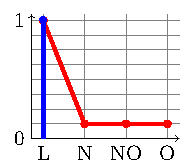
\includegraphics[width=\linewidth]{plot_tikz/speed1.pdf}
\caption{Initial}
\label{fig:a}
\end{subfigure}
\begin{subfigure}[t]{.15\linewidth}
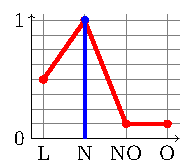
\includegraphics[width=\linewidth]{plot_tikz/speed12.pdf}
\caption{After 12 occurrences}
\label{fig:b}
\end{subfigure}
\begin{subfigure}[t]{.15\linewidth}
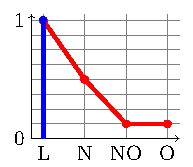
\includegraphics[width=\linewidth]{plot_tikz/speed17.pdf}
\caption{After 17 occurrences}
\label{fig:c}
\end{subfigure}
\begin{subfigure}[t]{.15\linewidth}
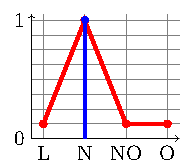
\includegraphics[width=\linewidth]{plot_tikz/speed22.pdf}
\caption{After 22 occurrences}
\label{fig:e}
\end{subfigure}
\begin{subfigure}[t]{.15\linewidth}
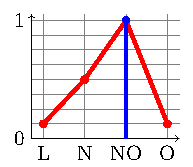
\includegraphics[width=\linewidth]{plot_tikz/speed24.pdf}
\caption{After 24 occurrences}
\label{fig:f}
\end{subfigure}
\begin{subfigure}[t]{.15\linewidth}
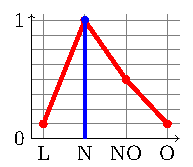
\includegraphics[width=\linewidth]{plot_tikz/speed27.pdf}
\caption{After 27 occurrences}
\label{fig:g}
\end{subfigure}
\\
\vspace{0.5cm}
\begin{subfigure}[b]{.15\linewidth}
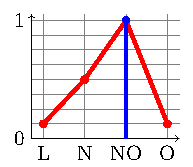
\includegraphics[width=\linewidth]{plot_tikz/speed28.pdf}
\caption{After 28 occurrences}
\label{fig:h}
\end{subfigure}
\begin{subfigure}[b]{.15\linewidth}
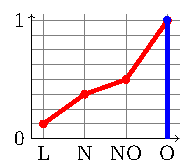
\includegraphics[width=\linewidth]{plot_tikz/speed29.pdf}
\caption{After 29 occurrences}
\label{fig:i}
\end{subfigure}
\begin{subfigure}[b]{.15\linewidth}
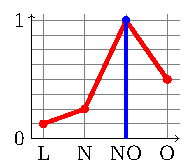
\includegraphics[width=\linewidth]{plot_tikz/speed30.pdf}
\caption{After 30 occurrences}
\label{fig:l}
\end{subfigure}
\begin{subfigure}[b]{.15\linewidth}
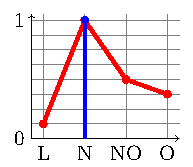
\includegraphics[width=\linewidth]{plot_tikz/speed31.pdf}
\caption{After 31 occurrences}
\label{fig:m}
\end{subfigure}
\begin{subfigure}[b]{.15\linewidth}
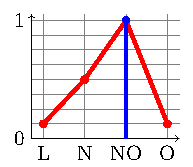
\includegraphics[width=\linewidth]{plot_tikz/speed33.pdf}
\caption{After 33 occurrences}
\label{fig:o}
\end{subfigure}
\begin{subfigure}[b]{.15\linewidth}
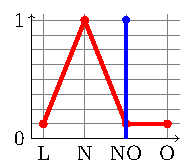
\includegraphics[width=\linewidth]{plot_tikz/speed28CONF.pdf}
\caption{After 34 occurrences}
\label{fig:speed34}
\end{subfigure}
\\
\vspace{0.5cm}
\caption[Possibilistic estimation on human assessment: experiment 1]{Experiment 1: Possibilistic estimation on human assessment of Airspeed (solid red curve), and actual machine state (blue bar). ``L'' is ``Low speed'', ``N'' is ``Normal speed'', ``NO'' is ``Near Overspeed'' and ``O'' is Overspeed.}
\label{fig:SpeedB}
\end{figure}

%\begin{figure}
%\centering
%\subfloat[\footnotesize  ]{\label{fig:a}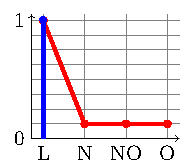
\includegraphics[width=0.41\linewidth]{plot_tikz/speed1.pdf}}  \hspace{0.3cm}
%\subfloat[\footnotesize ]{\label{fig:b}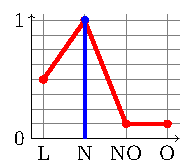
\includegraphics[width=0.41\linewidth]{plot_tikz/speed12.pdf}}\\
%\vspace{-0.15cm}
%\subfloat[\footnotesize After 17 occurrences ]{\label{fig:c}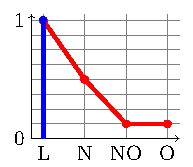
\includegraphics[width=0.41\linewidth]{plot_tikz/speed17.pdf}} \hspace{0.3cm}
%\subfloat[\footnotesize After 22 occurrences ]{\label{fig:e}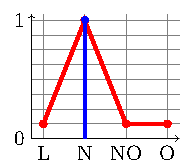
\includegraphics[width=0.41\linewidth]{plot_tikz/speed22.pdf}}\\
%\vspace{-0.15cm}
%\subfloat[\footnotesize After 24 occurrences]{\label{fig:f}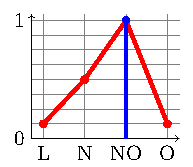
\includegraphics[width=0.41\linewidth]{plot_tikz/speed24.pdf}} \hspace{0.3cm}
%\subfloat[\footnotesize After 27 occurrences]{\label{fig:g}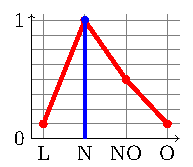
\includegraphics[width=0.41\linewidth]{plot_tikz/speed27.pdf}} \\
%\vspace{-0.15cm}
%\subfloat[\footnotesize After 28 occurrences]{\label{fig:h}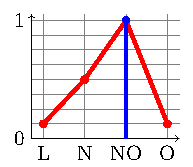
\includegraphics[width=0.41\linewidth]{plot_tikz/speed28.pdf}} \hspace{0.3cm}
%\subfloat[\footnotesize After 29 occurrences]{\label{fig:i}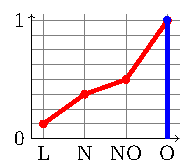
\includegraphics[width=0.41\linewidth]{plot_tikz/speed29.pdf}}\\
%\vspace{-0.15cm}
%\subfloat[\footnotesize After 30 occurrences]{\label{fig:l}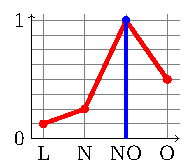
\includegraphics[width=0.41\linewidth]{plot_tikz/speed30.pdf}} \hspace{0.3cm}
%\subfloat[\footnotesize After 31 occurrences ]{\label{fig:m}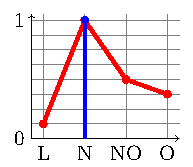
\includegraphics[width=0.41\linewidth]{plot_tikz/speed31.pdf}}\\
%\vspace{-0.15cm}
%\subfloat[\footnotesize After 33 occurrences]{\label{fig:o}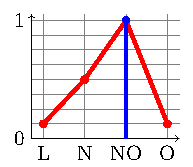
\includegraphics[width=0.41\linewidth]{plot_tikz/speed33.pdf}} \hspace{0.3cm}
%\subfloat[\footnotesize After 34 occurrences]{\label{fig:speed34}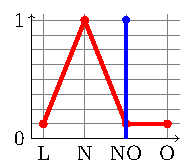
\includegraphics[width=0.41\linewidth]{plot_tikz/speed28CONF.pdf}}
%\caption{Experiment 1: Possibilistic estimation on human assessment of Airspeed (continuous red curve), and actual machine state (blue bar). ``L'' is ``Low speed'', ``N'' is ``Normal speed'', ``NO'' is ``Near Overspeed'' and ``O'' is Overspeed.}
%\label{fig:SpeedB}
%\end{figure}

The sequence of occurrences 
generated from the data 
recorded during the experience 
with the first participant 
is shown hereafter. 
A total of $57$ occurrences 
(among which are some selections) 
have been generated:

%\begin{framed}
\begin{footnotesize}
`Initialization', `Control Stick Off', `Throttle lever On', `Throttle lever Off', `Throttle lever On', `Throttle lever Off', `Throttle lever On', `Throttle lever Off', `Throttle lever On', `Throttle lever Off', `Control Stick On', `Speed Normal', `Control Stick Off', `Control Stick On', `ATHR button', `Control Stick Off', `SpeedLow', `Speed Normal', `Control Stick On', `Control Stick Off', `Control Stick On', `AP button', `Control Stick Off', `Near overspeed', `Control Stick On', `Control Stick Off', `Speed Normal', `Near overspeed', `Overspeed', `Near overspeed', `Speed Normal', `AP button', `Near overspeed', `Trajectory divergence',  `AP button', `Control Stick On',  `Control Stick Off', `Control Stick On', `Control Stick Off', `Control Stick On', `Control Stick Off', `Control Stick On', `Control Stick Off', `Control Stick On', `Control Stick Off', `Control Stick On', `Control Stick Off', `Control Stick On', `Control Stick Off', `AP button', `Trajectory divergence', `AP button', `Control Stick On', `Speed Normal', `Near overspeed', `Control Stick Off'
\end{footnotesize}
%\end{framed}


%\begin{framed}
%\begin{footnotesize}
%`Initialization', `Control Stick Off', `Throttle lever On', `Throttle lever Off', `Throttle lever On', `Throttle lever Off', `Throttle lever On', `Throttle lever Off', `Throttle lever On', `Throttle lever Off', `Control Stick On', `Speed Normal', `Control Stick Off', `Control Stick On', `ATHR button', `Control Stick Off', `SpeedLow', `Speed Normal', `Control Stick On', `Control Stick Off', `Control Stick On', `AP button', `Control Stick Off', `Near overspeed', `Control Stick On', `Control Stick Off', `Speed Normal', `Near overspeed', `Overspeed', `Near overspeed', `Speed Normal', `AP button', `Near overspeed', `Trajectory divergence',  `AP button', `Control Stick On',  `Control Stick Off', `Control Stick On', `Control Stick Off', `Control Stick On', `Control Stick Off', `Control Stick On', `Control Stick Off', `Control Stick On', `Control Stick Off', `Control Stick On', `Control Stick Off', `Control Stick On', `Control Stick Off', `AP button', `Trajectory divergence', `AP button', `Control Stick On', `Speed Normal', `Near overspeed', `Control Stick Off'
%\end{footnotesize}
%\end{framed}

The initial machine state is:
\begin{description}
\item $s_1=$ AP state: Off;
\item $s_2=$ ATHR state: On;
\item $s_3=$ Airspeed: Underspeed;
\item $s_4=$ Control stick: Actioning;
\item $s_5=$ Throttle lever:  Not actioning.
\end{description}
After the firing of the $25$th occurrence, 
$119.5$ seconds from the beginning of the experiment, 
the analysis model detects an exception:
\begin{description}
\item \texttt{Exception description: `Control stick On when AP on!'}.
\end{description}
After the firing of the $34$th occurrence, 
$772.6$ seconds from the beginning of the experiment, 
the analysis model detects an exception and explains it:
\begin{description}
\item \texttt{Exception description: `Vertical speed divergence $>$ 250 ft, unnoticed' because 'Speed becomes $>$Vmax-5, but unseen!'}.
\end{description}

After the firing of the $51$st occurrence, 
$886.1$ seconds from the beginning of the experiment, 
an exception is explained again:
\begin{description}
\item \texttt{Exception description: `Vertical speed divergence $>$ 250 ft, unnoticed' because 'Speed becomes $>$Vmax-5, but unseen!'}.
\end{description}
It is worth noting that the experimenters \cite{pizziol14} 
reported two human automation conflicts 
corresponding to the second and third exceptions, 
and that their findings on those conflicts causes 
(based on the observation of the data, 
the video recording and the interview of the pilot) 
is in agree with the exception explanation provided 
by the analysis model here.

After the execution of the $57$ occurrences, 
$196$ assessment trajectories are considered as possible 
(with different possibility degrees). 
The computation time is $30$ seconds. 
Some possibilistic estimations of the human assessment of the machine state 
variable ``Airspeed''
are represented in Figure \ref{fig:SpeedB}:
the possibility distribution over the human assessment $h$
of the airspeed, $\pi_t(h)$, is indicated by the red curve. 
This possibilistic evaluation is qualitative, 
nevertheless in the graphic representation, 
quantitative values are arbitrarily assigned 
to the possibility degrees 
(respecting qualitative ordering) to plot them. 
The actual machine state $s$ is stated 
by the blue bar with value $1$ on the y-axis:
if no exception arises, most possible assessment $h$ 
should be the actual state (blue bar). 
%Moreover 
%the second most possible estimate should be the former value (prior to the last fired occurrence) 
%of the actual state. The third most possible estimate should be the value of the actual state prior to the last two changes and so on.

%\begin{figure}
%\centering
%\subfloat[\footnotesize Initial ]{\label{fig:a}\includegraphics[width=0.5\linewidth]{Speed1.png}}  
%\subfloat[\footnotesize After 12 occurrences]{\label{fig:b}\includegraphics[width=0.5\linewidth]{Speed12.png}}\\

%\subfloat[\footnotesize After 17 occurrences ]{\label{fig:c}\includegraphics[width=0.5\linewidth]{Speed17.png}}  
%\subfloat[\footnotesize After 22 occurrences ]{\label{fig:e}\includegraphics[width=0.5\linewidth]{Speed22.png}}\\

%\subfloat[\footnotesize After 24 occurrences]{\label{fig:f}\includegraphics[width=0.5\linewidth]{Speed24.png}} 
%\subfloat[\footnotesize After 27 occurrences]{\label{fig:g}\includegraphics[width=0.5\linewidth]{Speed27.png}} \\

%\subfloat[\footnotesize After 28 occurrences]{\label{fig:h}\includegraphics[width=0.5\linewidth]{Speed28.png}}
%\subfloat[\footnotesize After 29 occurrences]{\label{fig:i}\includegraphics[width=0.5\linewidth]{Speed29.png}}\\

%\subfloat[\footnotesize After 30 occurrences]{\label{fig:l}\includegraphics[width=0.5\linewidth]{Speed30.png}}
%\subfloat[\footnotesize After 31 occurrences ]{\label{fig:m}\includegraphics[width=0.5\linewidth]{Speed31.png}}\\

%\subfloat[\footnotesize After 33 occurrences]{\label{fig:o}\includegraphics[width=0.5\linewidth]{Speed33.png}}
%\subfloat[\footnotesize After 34 occurrences]{\label{fig:speed34}\includegraphics[width=0.5\linewidth]{Speed28CONF.png}}
%\caption{Speed possibility distribution, {\color{blue} blue actual (s)}, {\color{red} red estimation (h)} }
%\label{fig:SpeedB}
%\end{figure}



Remember that after the firing of $34$ occurrences 
an exception is detected by the analysis model, 
which is graphically highlighted in Figure \ref{fig:speed34}: 
most possible human assessment is no more the real machine state.
% the objective assessment trajectory is no longer considered as normal\footnote{The possibility for a normal occurrence is 1.}. 
%Also after an exception the most possible estimation for the human assessment of the internal state (which is wrong in this case) is given by the maximum of the red line.

\subsubsection{Example 2}


\begin{figure}\centering
\begin{subfigure}[t]{.15\linewidth}
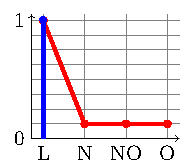
\includegraphics[width=\linewidth]{plot_tikz/speed1.pdf}
\caption{Initial}
\label{fig:a}
\end{subfigure}
\begin{subfigure}[t]{.15\linewidth}
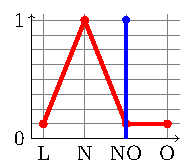
\includegraphics[width=\linewidth]{plot_tikz/speed28CONF.pdf}
\caption{After 18 occurrences}
\label{fig:b}
\end{subfigure}
\begin{subfigure}[t]{.15\linewidth}
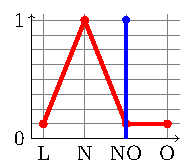
\includegraphics[width=\linewidth]{plot_tikz/speed28CONF.pdf}
\caption{After 46 occurrences}
\label{fig:c}
\end{subfigure}
\begin{subfigure}[t]{.15\linewidth}
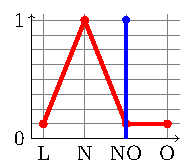
\includegraphics[width=\linewidth]{plot_tikz/speed28CONF.pdf}
\caption{After 49 occurrences}
\end{subfigure}
\\
\vspace{0.5cm}
\caption[Possibilistic estimation on human assessment: experiment 2]{Experiment 2: Possibilistic estimation on human assessment of speed (solid red curve), actual machine state (blue bar).}
\label{fig:SpeedC}
\end{figure}


A sequence of occurrences has been generated 
from the data recorded during experience 
with a second participant. 
A total of $85$ occurrences (among which are some human selections) have been generated. 
Hereafter the beginning of the sequence:

%\begin{framed}
\begin{footnotesize}
`Initialization', `Throttle lever On', `Throttle lever Off', `ATHR button', `Throttle lever On' ...
\end{footnotesize}
%\end{framed}

%
%:
%
%\begin{framed}
%\begin{footnotesize}
%`Initialization', 'Throttle lever On', `Throttle lever Off', `ATHR button', `Control Stick On', `Throttle lever On', `Throttle lever Off', `ATHR button', `ATHR button', `Control Stick Off', `Control Stick On', `ATHR button', `Control Stick Off', `Speed Normal', `Control Stick On', `Control Stick Off', `AP button', `Near overspeed', `Speed Normal', `Near overspeed', `Overspeed', `Near overspeed', `Overspeed', `Near overspeed', `Speed Normal', `Control Stick On', `Control Stick Off', `Control Stick On', `Control Stick Off', `Control Stick On', `Control Stick Off', `Control Stick On', `Near overspeed', `Speed Normal', `Near overspeed', `Speed Normal', `Near overspeed', `Speed Normal', `Near overspeed', `Overspeed', `Near overspeed', `Control Stick Off', `Speed Normal', `AP button', `Near overspeed', `ATHR button', `exceedingVzLevel1', `Throttle lever On', `Throttle lever Off', `Throttle lever On', `Throttle lever Off', `Throttle lever On', `Throttle lever Off', `Throttle lever On', `Throttle lever Off', `Control Stick On', `Speed Normal', `Control Stick Off', `Throttle lever On', `Throttle lever Off', `Throttle lever On', `Throttle lever Off', `Throttle lever On', `Throttle lever Off', `Throttle lever On', `Throttle lever Off', `Throttle lever On', `Throttle lever Off', `Throttle lever On', `Throttle lever Off', `Throttle lever On', `Throttle lever Off', `Throttle lever On', `Throttle lever Off', `Throttle lever On', `Throttle lever Off', `Throttle lever On', `Throttle lever Off', `Throttle lever On', `Throttle lever Off', `Throttle lever On', `Throttle lever Off', `Throttle lever On', `Throttle lever Off', `ATHR button'
%\end{footnotesize}
%\end{framed}

Initial machine state variables are the same as previously, 
except of control stick, which is here initially actioning.
%%\vspace{-0.7\baselineskip} 
%\begin{description}
%\item AP state: Off
%\item ATHR state: On
%\item  Airspeed: Underspeed
%\item Control stick:  Not actioning
%\item  Throttle lever:  Not actioning
%\end{description}
%%\vspace{-0.7\baselineskip} 

%\begin{figure}[t!]
%%\vspace{-\baselineskip} 
%\centering
%\subfloat[\footnotesize Initial ]{\label{fig:a}\includegraphics[width=0.5\linewidth]{Speed1.png}}  
%\subfloat[\footnotesize After 18 occurrences]{\label{fig:b}\includegraphics[width=0.5\linewidth]{Speed28CONF.png}}\\
%\vspace{-0.4cm}
%\subfloat[\footnotesize After 46 occurrences ]{\label{fig:c}\includegraphics[width=0.5\linewidth]{Speed28CONF.png}}  
%\subfloat[\footnotesize After 49 occurrences]{\label{fig:d}\includegraphics[width=0.5\linewidth]{Speed28CONF.png}}\\
%\caption{Speed possibility distribution, {\color{blue} blue actual (s)}, {\color{red} red estimation (h)} }
%\label{fig:SpeedC}
%\end{figure}




This second example was chosen because of the second occurrence, 
$30.2$ seconds from the beginning of the experiment.
The analysis model detects the following exception:
\begin{description}
\item \texttt{Exception description: `Throttle lever On when ATHR on!' because 'Wrong state initialization'}
\end{description}
Initially the ATHR is on: operating the throttle lever has no result 
(this action is considered as a slip). 
The model explains this slip as the result of a wrong initial assessment: 
if the pilot initial assessment of the ATHR state was Off, 
that could explain the execution of this action as nominal. 
It is worth noting that after giving up this useless action (`Throttle lever Off') 
the participant deactivated the ATHR (`ATHR button') 
and she/he started again operating the throttle lever ('Throttle lever On'), 
probably because she/he had a wrong initial situation assessment 
(as the found exception explanation) and she/he understood their assessment error. 

%\begin{figure}[t!]
%\centering
%\subfloat[\footnotesize Initial ]{\label{fig:a}\includegraphics[width=0.5\linewidth]{marpaATHRstate1.png}}  
%\subfloat[\footnotesize After 2 occurrences]{\label{fig:b}\includegraphics[width=0.5\linewidth]{marpaATHRstate2.png}}\\
%\caption{ATHR state possibility distribution.}
%\label{fig:ATHR}
%%\vspace{-\baselineskip} 
%\end{figure}
The analysis model detected also three times the same exception as for the previous participant:
\begin{description}
\item \texttt{Exception description: `Vertical speed divergence $>$ 250 ft, unnoticed' because 'Speed becomes $>$Vmax-5, but unseen!'}
\end{description}
Figure \ref{fig:SpeedC} shows the estimation of the human assessment 
of the speed, initially, and when these exceptions occur.

\section{Conclusion}
This chapter proposes a model for the human-machine interaction based 
on a machine model and expert knowledge on an human assessment error model.
The human-machine interaction is modelled as a possibilistic hidden Markov process. 
Qualitative Possibility Theory has been chosen because 
it is well suited to handle uncertainty defined by expert knowledge. 
The proposed possibilistic analysis model provides 
an estimation of the human assessment of the machine state 
and detects assessment errors. 
The analysis model is able to provide also an explanation (diagnosis) 
when an assessment error is detected.

This process of detection/identification 
could be used in real time applications in order to 
inform the human operator of their assessment errors.
It can help to make them correct their situation awareness 
and prevent the execution of other errors.

This work is based on the simplifying assumption 
that the human operator is certain about the state 
of the machine: a possible extension of this model 
may be to drop this assumption using a more refined 
representation of the human state assessment, 
as a set of machine states, or an uncertainty 
measure over the machine states.

This article proposes a model for the human-machine interaction based 
on a machine model and expert knowledge on an human assessment error model.
The human-machine interaction is modelled as a possibilistic hidden Markov process. 
Qualitative Possibility Theory has been chosen because 
it is well suited to handle uncertainty defined by expert knowledge. 
The proposed possibilistic analysis model provides 
an estimation of the human assessment of the machine state 
and detects assessment errors. 
The analysis model is able to provide also an explanation (diagnosis) 
when an assessment error is detected.

This process of detection/identification 
could be used in real time applications in order to 
inform the human operator of their assessment errors.
It can help to make them correct their situation awareness 
and prevent the execution of other errors.

This work is based on the simplifying assumption 
that the human operator is certain about the state 
of the machine: a possible extension of this model 
may be to drop this assumption using a more refined 
representation of the human state assessment, 
as a set of machine states, or an uncertainty 
measure over the machine states.

